\documentclass[a4paper, 9pt]{article}
\usepackage{nips15submit_e}
\usepackage{graphicx}
\usepackage{amssymb}
\usepackage{float}
\graphicspath{}
\usepackage[margin=1in]{geometry}
\title{Machine Learning Coursework 1}
\author{
    Elizabeth Tebbutt (et15611), Aidan Ball (ab15100),
    \And Esta Cooksley (ec15201), Tom Vaughan (tv15461)
}
\begin{document}
\maketitle
\section*{Question 1}
\subsection*{Why is choosing a Gaussian likelihood a sensible thing to do?}
If we assume that our two points are iid, thanks to the central limit theorem we know that the average of iid samples from any distribution will follow a Gaussian distribution with the mean tending towards the mean of the sample population. Thus we can assume that our curve is Gaussian with a peak at the mean, which would be the mapping over x as without error this is what we would pick to be most likely as the outcome. It does not vary if we are assuming the mapping is linear. We have to take into account error, which can vary, and in this case the error would be additive; this makes it sensible to be the variance. This along with the fact that our mean is the mapping over x means that we can use the Gaussian distribution: \\

\( N(f(x_i), \sigma^2 \mathbf{I} ) \) \\

It's also worth noting that Gaussian distributions are easy to work with, as a Gaussian prior also has a Gaussian conjugate and posterior.
\subsection*{What does it mean that we have chosen a spherical covariance matrix for the likelihood?}
A covariance matrix is spherical if it is proportional to the identity matrix. By choosing this we are assuming that each parameter has the same variance and there is 0 covariance (everything is independent) because we have no information to predict the relationship between the two. The distribution will show up as a perfect circle in 2D, a sphere in 3D, and so on.

\section*{Question 2}
\subsection*{If we do not assume that the data points are independent how would the likelihood look?}
The probability of some three parameters is \( P(x,y,z) \) and if these are independent: \\
\newline
\( p(x,y,z)=p(x)p(y)p(z) \) \\
\newline
If x and y change with z, \( P(x,y \mid z) \), we can use the product rule to get the following: \\
\newline
\( P(x,y,z) = P (x,y \mid z)P(z) \) \\
\newline
If x also depends on y, we can iterate again: \\
\newline
 \( P(x,y,z) = P(x \mid y,z)P(y \mid z)P(z) \) \\
 \newline
For large spaces with many more than three variables the dependencies become very messy and difficult to calculate, as over \( x_{0}...x_{n} \) elements  the number of times we have to apply the chain rule increases exponentially.

\section*{Question 3}
\subsection*{What is the specific form of the likelihood "above"?}
\( P( Y \mid X, W) = \prod N(wx, \epsilon) \) \\
This is true under the assumptions that x and y are iid.

\section*{Question 4}
\subsection*{Explain the concept of conjugate distributions. Why is this a motivated choice?}
Bayes theorem takes the form: \\
\newline
\( Posterior = \frac{likelihood \times prior}{evidence} \) \\
\newline
For some prior, we want the posterior to take the functional form of: \\
\newline
\( Posterior \propto likelihood \times prior \) \\
\newline
Because the evidence is very difficult to handle. \\
\newline
If the posterior is in the same family as the prior, then they are conjugate distributions. Thus, we need a prior which is conjugate to the likelihood, so the posterior and prior take the same form. \\
Conjugate distributions are very useful as if the posterior and prior are in the same form, we can put the new posterior back into the equation as a new prior, and iterate to improve the model very quickly and analysis is considerably simplified.

\section*{Question 5}
\subsection*{\( L_{1} \) vs \( L_{2} \) when encoding the preference}
An L1-norm loss function, known as least absolute deviations or least absolute errors, basically minimises the sum of the absolute differences between the target value and the estimated value. L2-norm functions, known as least squares error, minimise the sum of the square of the differences between the target value and estimated value. The fundamental difference between the two is the square!
For a spherical distribution, the L2 norm is just a straight line - there is only one solution. However, the L1 distribution may have multiple solutions.

\section*{Question 6}
\subsection*{Deriving the posterior over the parameters}
The posterior takes the form, \( (W \mid X, Y) \propto P(Y \mid W, X) \times P(W) \). Our prior is \( N(w_{0} ,\tau^{2} I) \), and our likelihood was defined in question 3. Thus to get our posterior \( N(w', a) \) we multiply the exponential forms of these together and simplify to reach Gaussian form, the exponent of this will reach a form A+B+C, where A is a constant term, B is a mixed term, and C has a quadratic in the parameters. We can then extract the mean from B by completing the square, then we use the schur complement to extract the variance from the entire exponent. The Z term normalises the function so that it becomes a distribution, i.e. sums to 1.  \\
This can be visualised as a line between the two means on a graph.

\section*{Question 7}
\subsection*{What is a non-parametric model. What is the difference between parametric and non parametric models?}
Parametric models assume that our parameters are finite in number; this inherently bounds the complexity of the model even if the amount of data provided is unbounded. This means they lack flexibility! However, they're easier to interpret as they're generally much simpler models. \\
Non-parametric models assume that the data distribution cannot be defined by a finite set of parameters; instead they are defined assuming an infinite dimensional dataset. The amount of data this model can capture increases as the quantity of data does, which makes them much more flexible. They are harder to interpret than parametric models, as it is over infinite space so cannot always be expressed.

\section*{Question 8}
\subsection*{Explain what "this" prior represents and how it places structure on the space of the functions.}
This prior states that we have a Gaussian distribution with mean 0 and a variance which is a function of X, which implies the variance changes with X and only with X. As the number of possible values of X is infinite, then the space the variance can cover is also infinite. If we assume nothing about X the variance encodes the data directly, while if we make an assumption this prior would reach the correct model very quickly.

\section*{Question 9}
\subsection*{Does "this" prior encode all possible functions or only a subset?}
This prior encodes all possible functions as a Gaussian never reaches 0, and both the variance and the model itself are Gaussian. Thus every single function can be represented, as the model covers infinite horizontal space and the variance covers infinite vertical space.

\section*{Question 10}
\subsection*{Formulating the joint distribution.}
Assuming the data is iid \\
\newline
Assuming a prior over the function, \( p (f \mid \theta) \), and a prior over the parameters, \(p(\theta ) \) \\
\newline
\( P(Y, X, f, \theta) = P(Y \mid X, f, \theta) \\
\newline
P(Y \mid f)P(f \mid \theta, X)P( \theta) \)\\
\begin{figure}[h]
\begin{center}
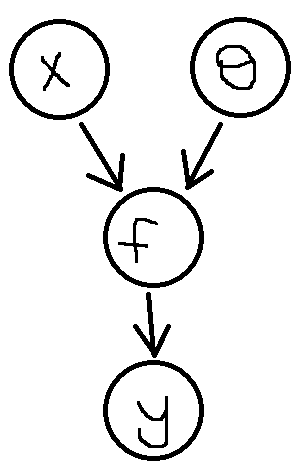
\includegraphics[width=0.6in,height=0.8in]{path}
\end{center}
\caption{Graphical Model}
\end{figure}

\section*{Question 11}
\subsection*{Explain the marginalisation in Eq.1.1.2}
In discrete space, to marginalise some data we need to multiply the data by its probability and add everything together; in continuous space this is done with integration. Marginalising this way allows us to find a distribution for a parameter y over some specific x, without having to take their relationship f into account at all. The uncertainty was initially contained in f, this has filtered through our function to be contained in the distribution y created for every x. We still have theta on the left side of the equation when we?re done; theta is the set of parameters in our covariance function k(X,X); this implies that the covariance function is still relevant to our marginalised belief.

\section*{Question 12}
The first plot is our prior over W, it is a simple bivariate gaussian.\\
\newline
\begin{figure}[H]
\begin{center}
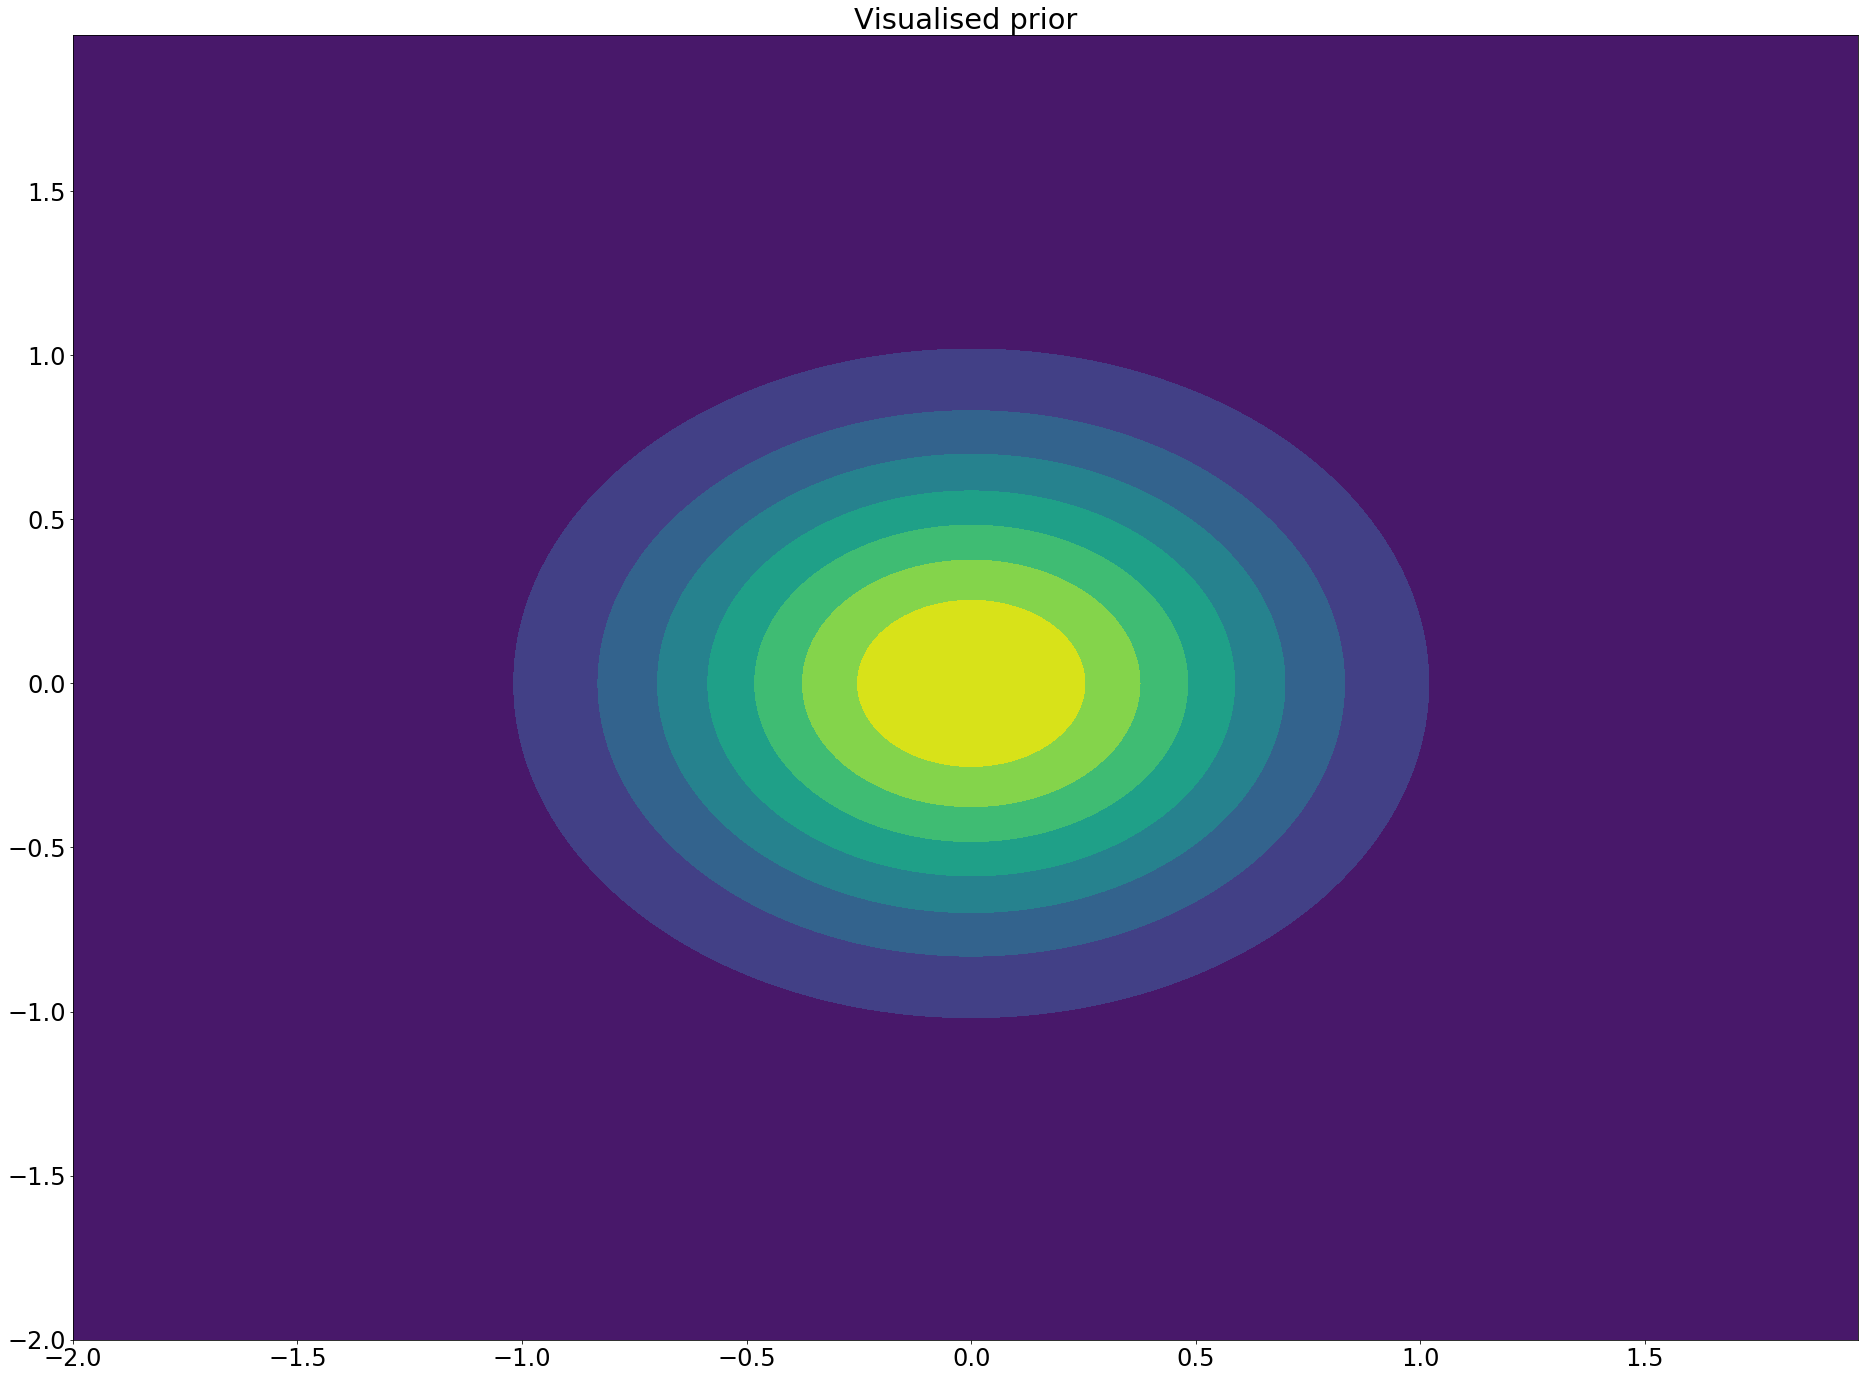
\includegraphics[width=1.8in,height=1.15in]{posterior0} \\
\end{center}
\caption{Prior over W}
\end{figure}
Having picked a data point, namely 0.89, we calculated the posterior distribution over W, you can see the prior over W and the posterior plotted here. We took a sample size of 1 over the functions.\\
\newline
\begin{figure}[H]
\begin{center}
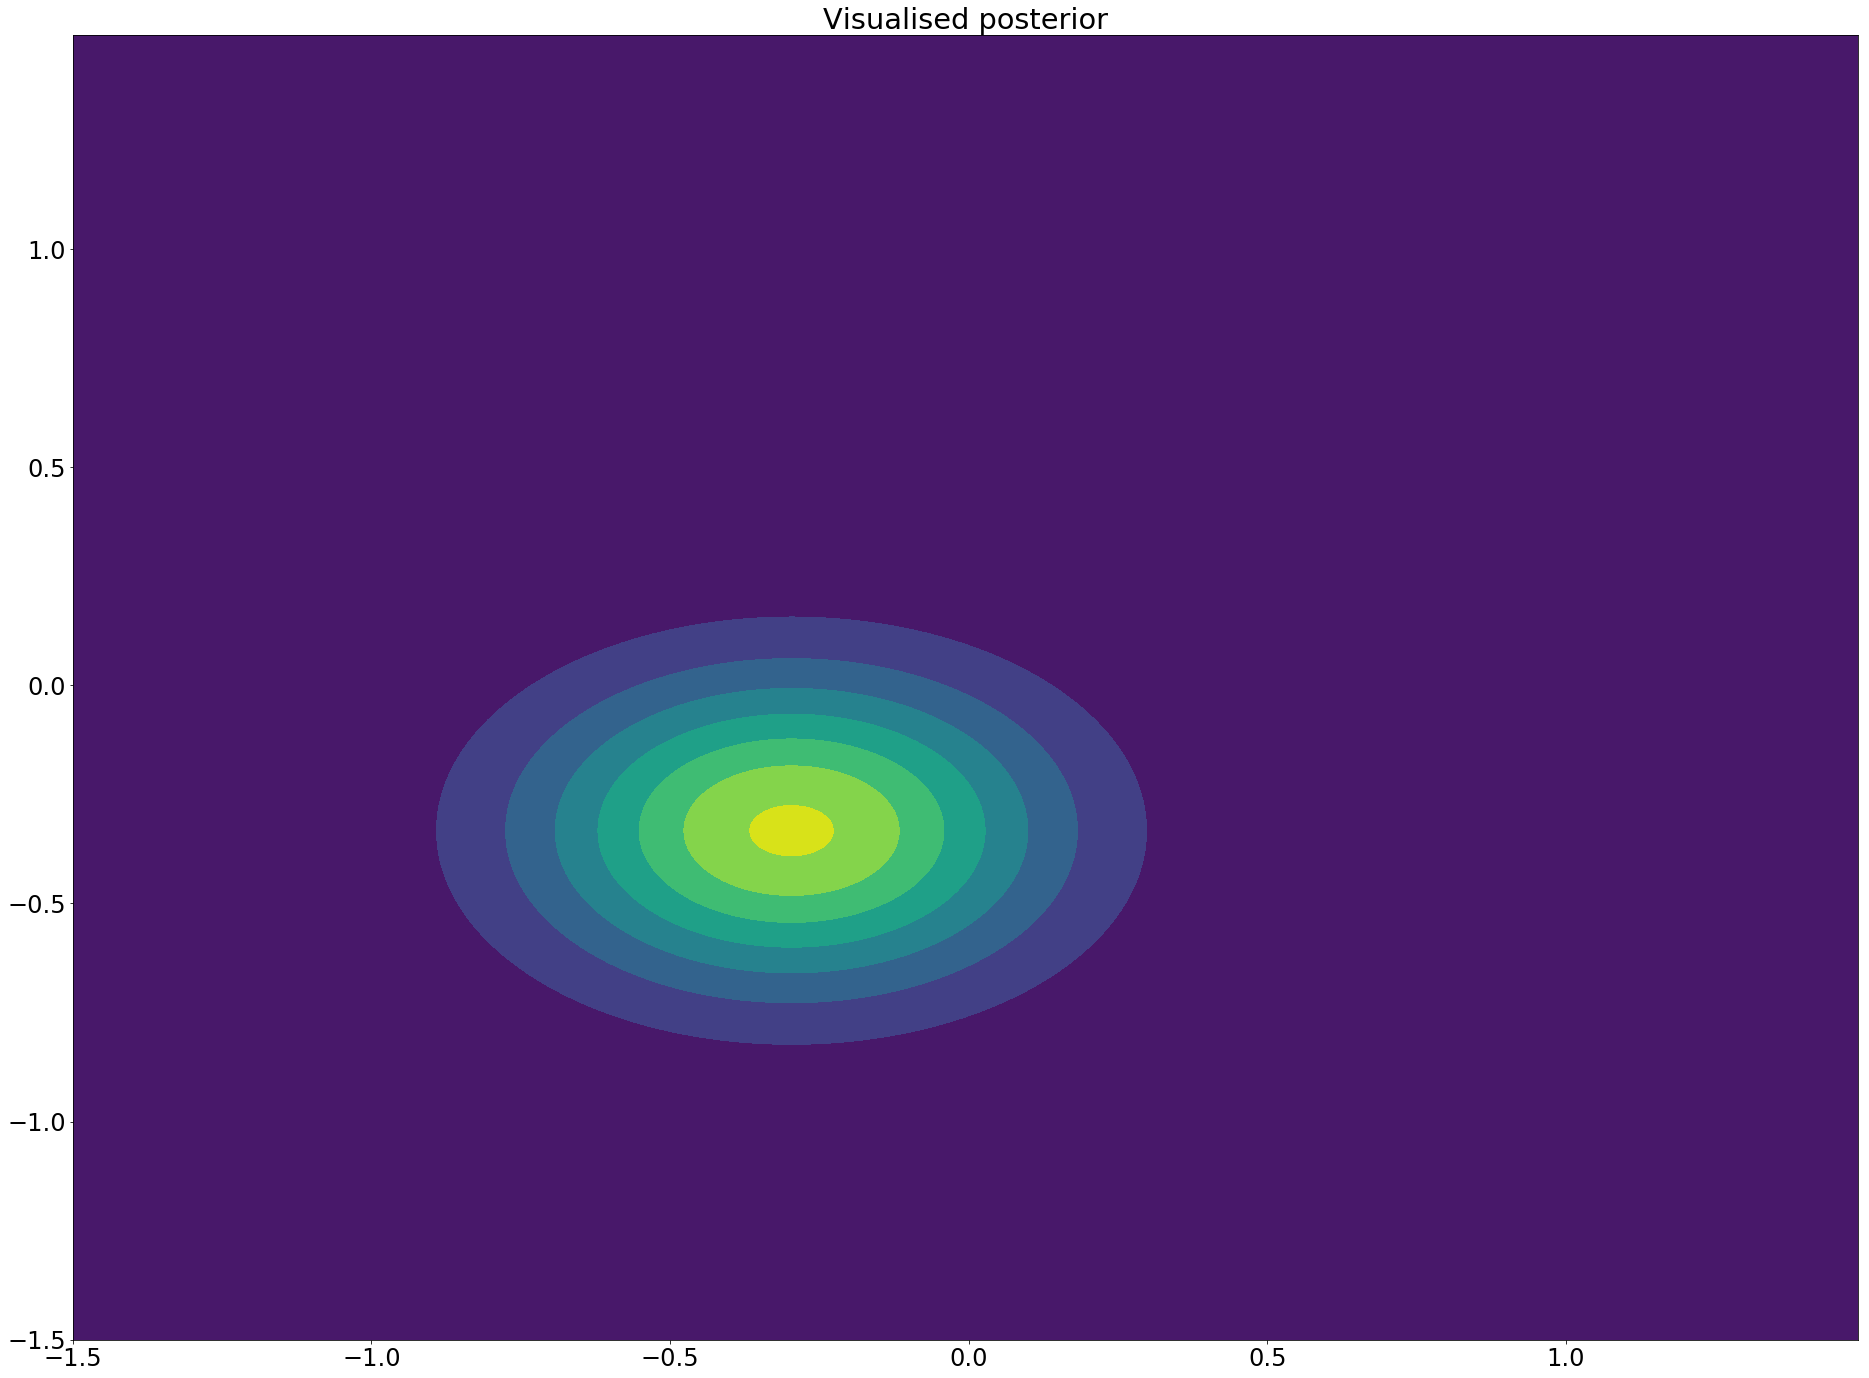
\includegraphics[width=1.8in,height=1.15in]{posterior1}
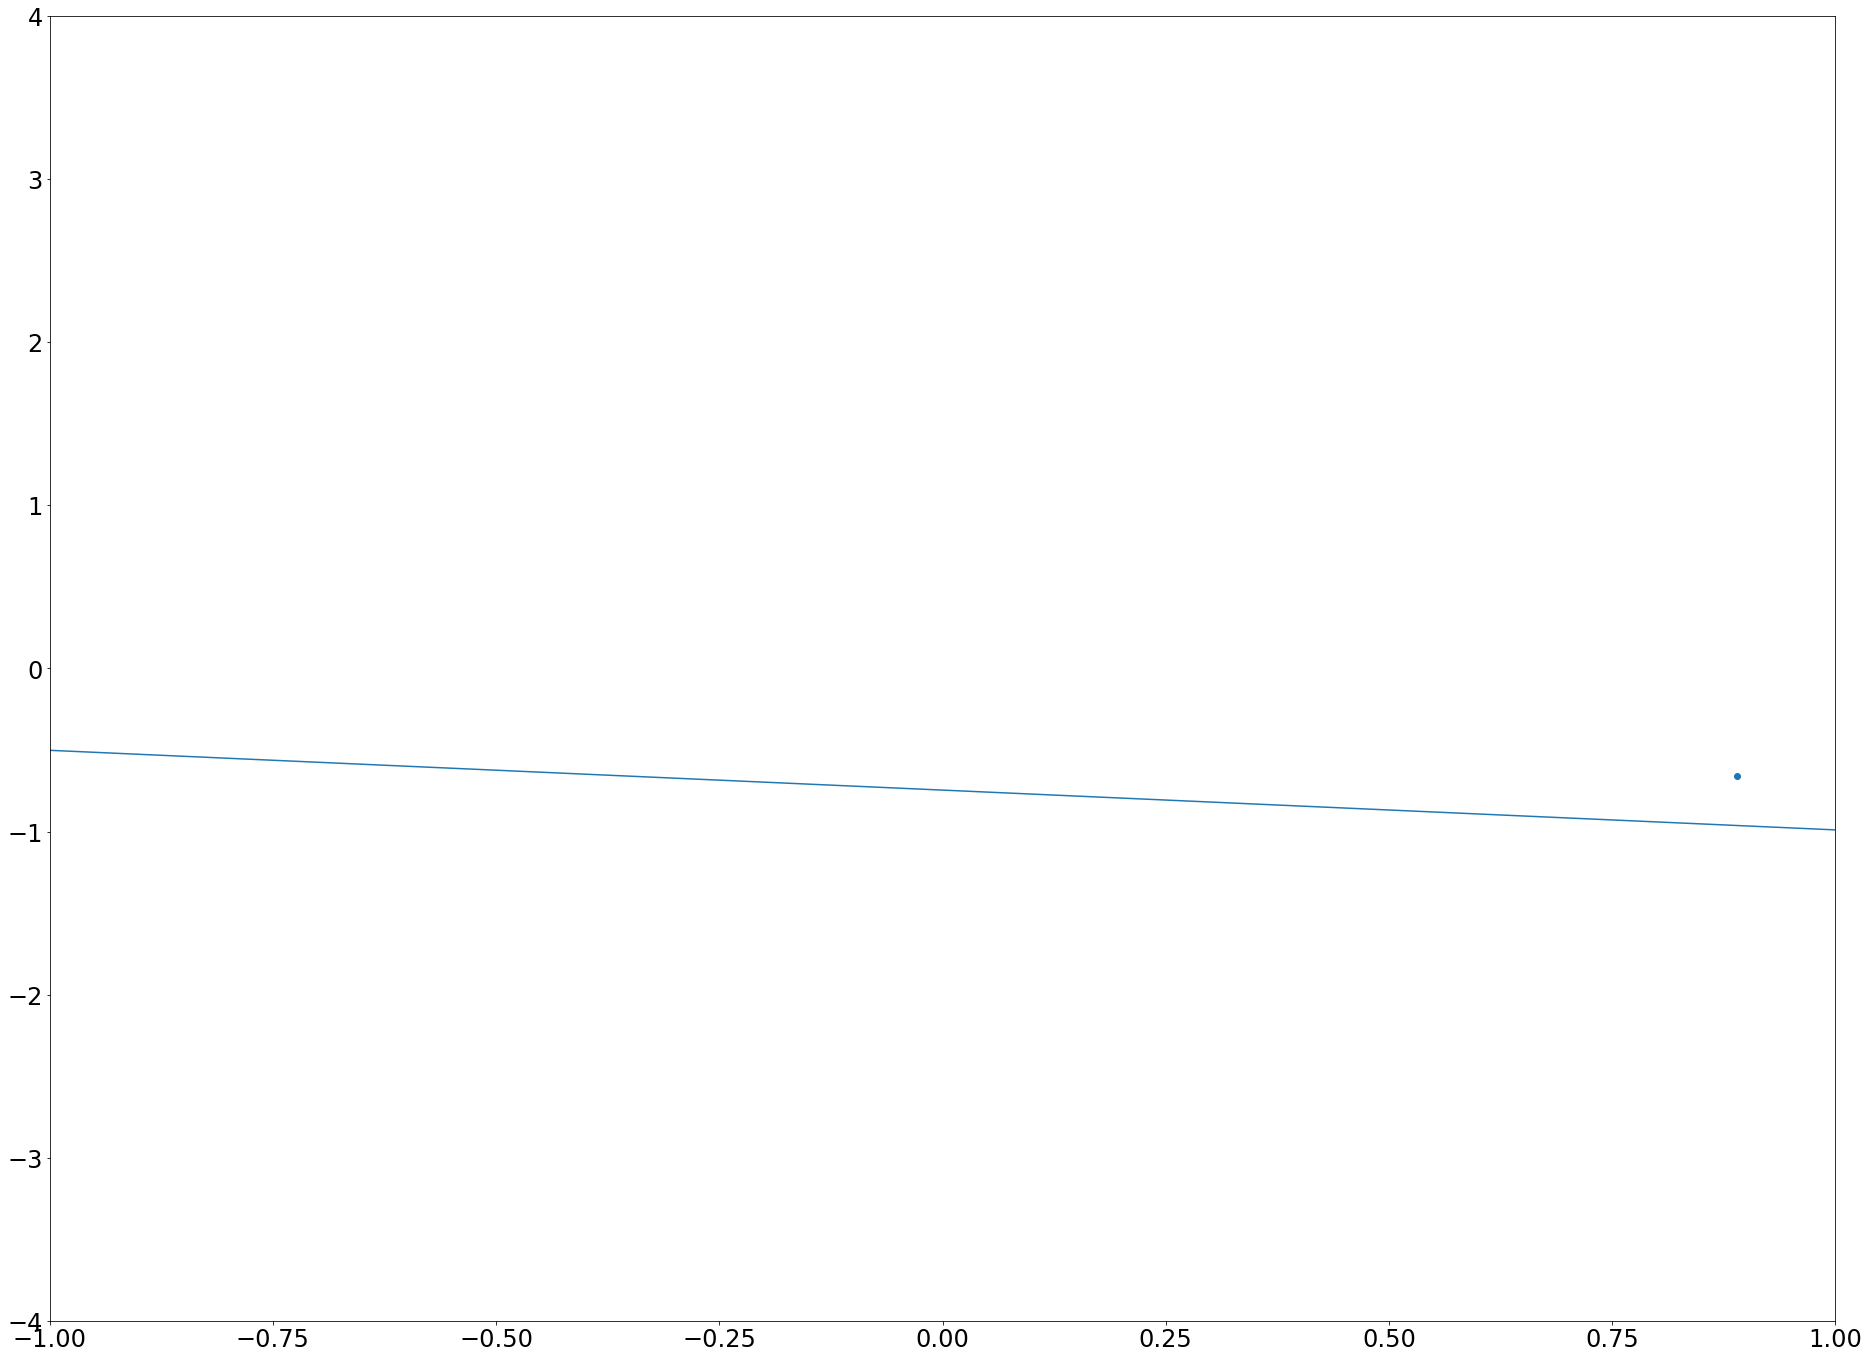
\includegraphics[width=1.8in,height=1.15in]{data1} \\
\end{center}
\caption{Posterior and Function after 1 Data Point}
\end{figure}
\begin{figure}[H]
\begin{center}
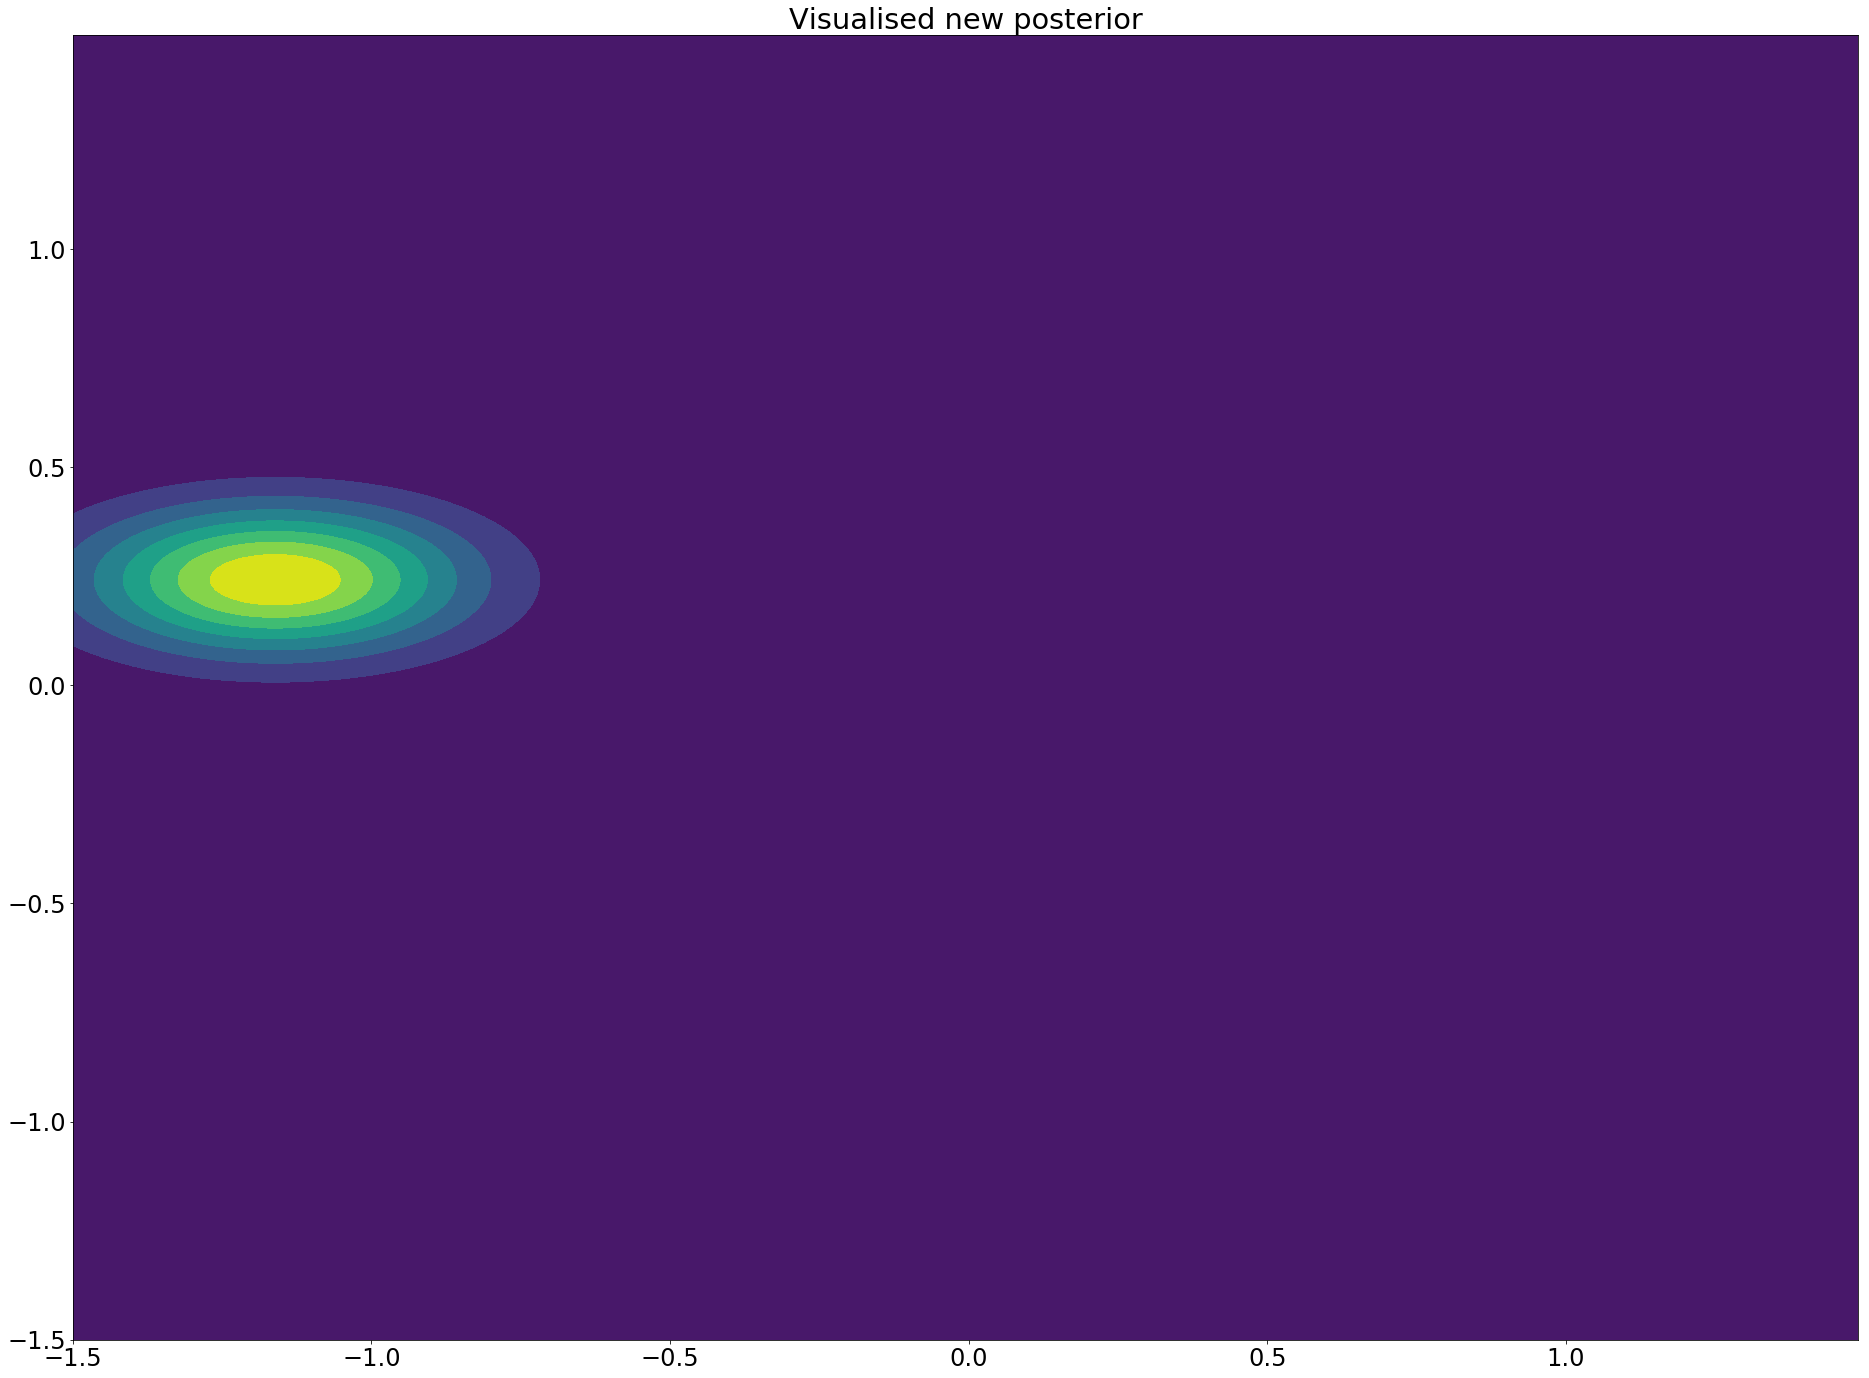
\includegraphics[width=1.8in,height=1.15in]{posterior2}
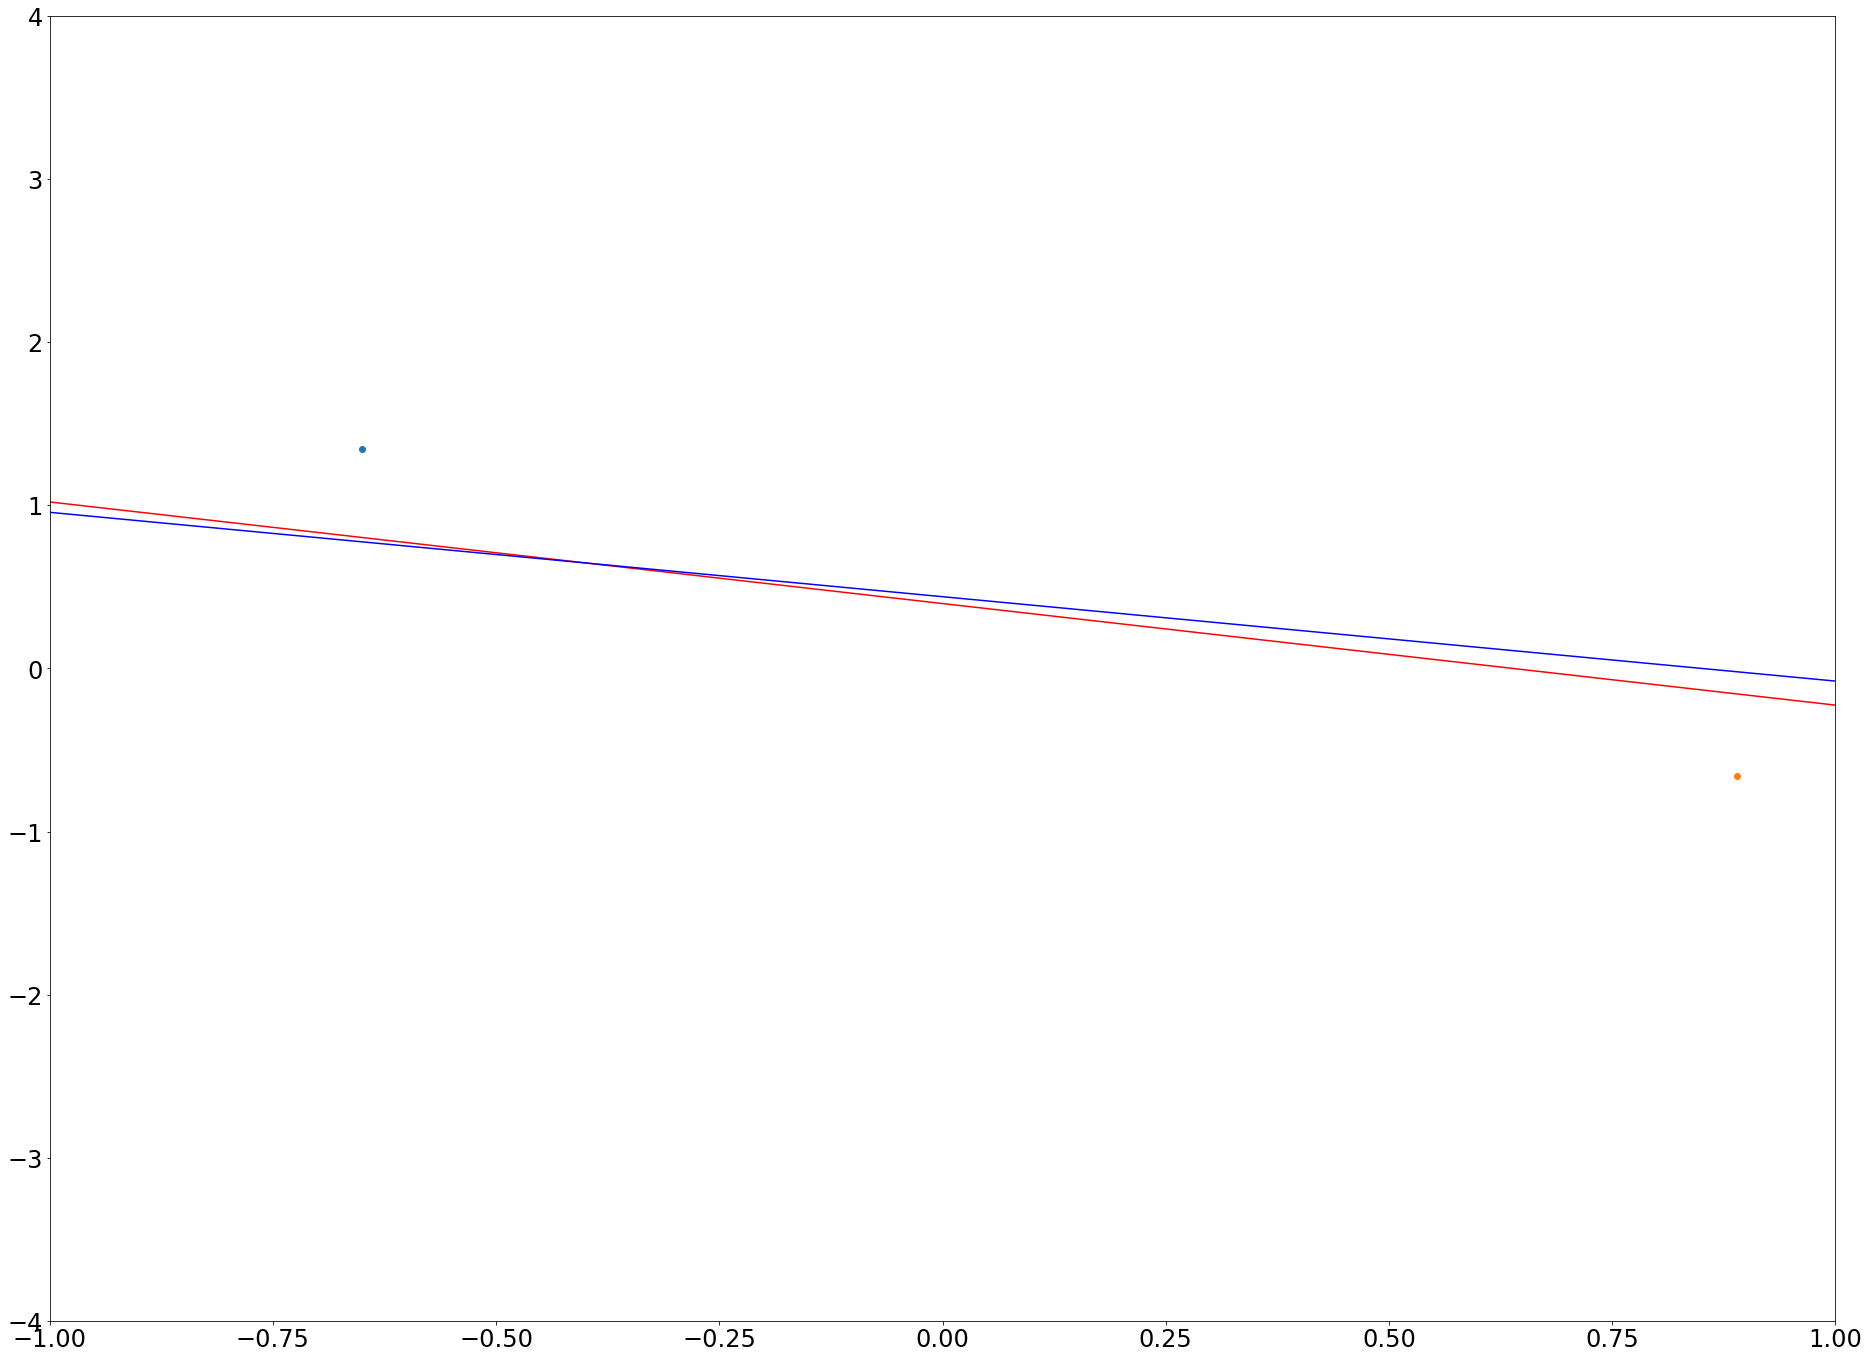
\includegraphics[width=1.8in,height=1.15in]{data2} \\
\end{center}
\caption{Posterior and Function after 2 Data Points}
\end{figure}
\begin{figure}[H]
\begin{center}
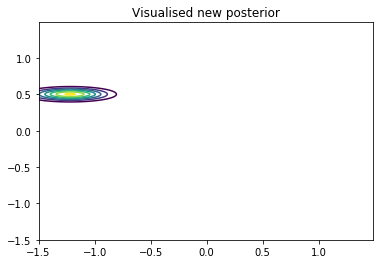
\includegraphics[width=1.8in,height=1.15in]{posterior3}
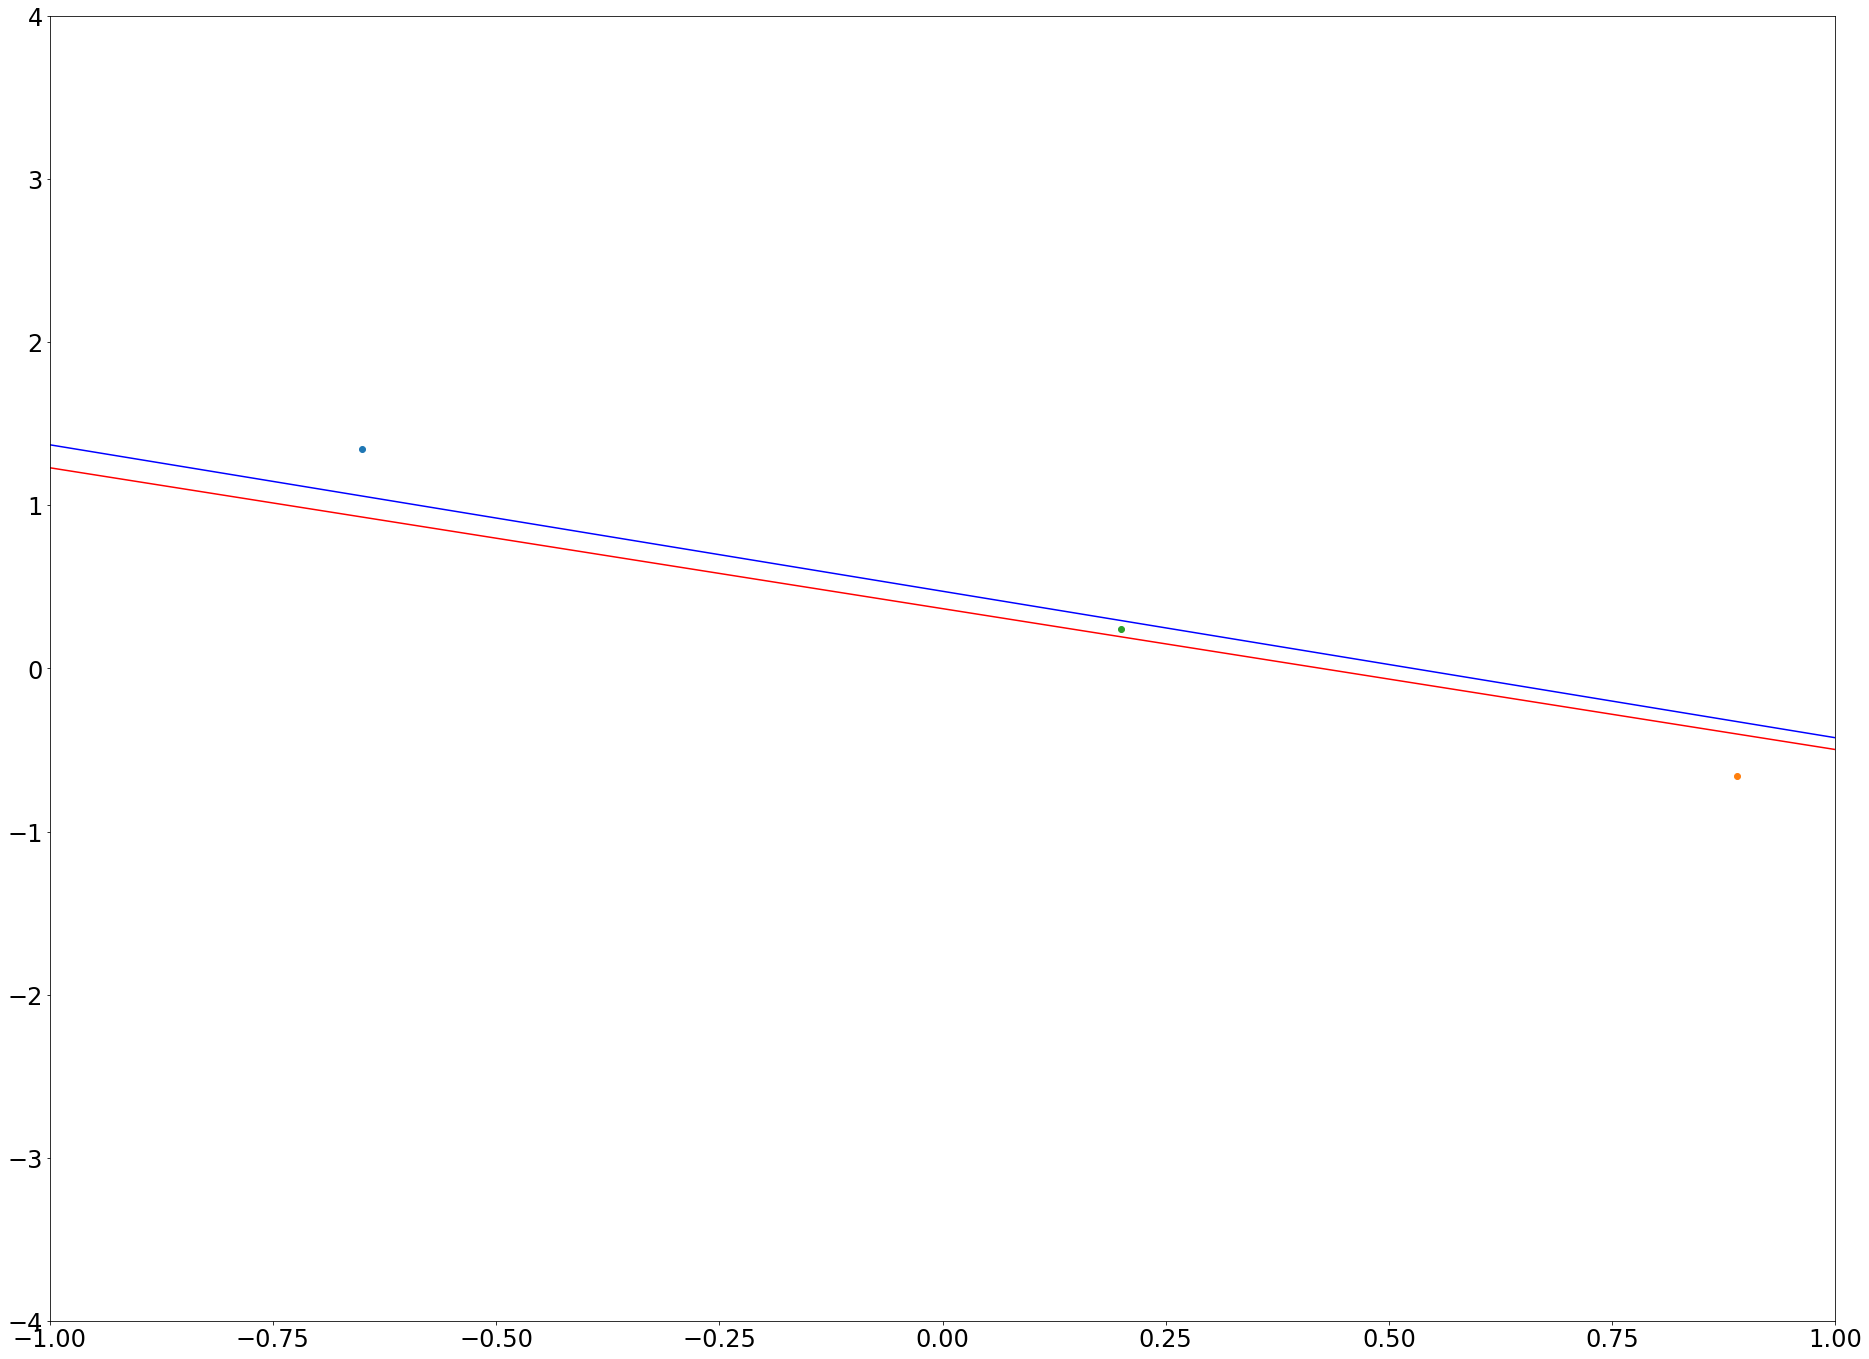
\includegraphics[width=1.8in,height=1.15in]{data3} \\
\end{center}
\caption{Posterior and Function after 3 Data Points}
\end{figure}

The graph with a point and a line, shows the point we chose, and a function sampled from the posterior generated. This is repeated for subsequent extra points.
As more data is added the posterior sampled functions becomes more likely to fit the data as a straight line, a line of best fit, which we an see happening in the figures. For a function that we strongly believe is linear this is desirable behaviour, but if our assumption of linear-ness is wrong, this would be quite damning.

\section*{Question 13}
For this question we had to create a gp prior using the squared covariance function as its kernel. You can see the GP we encoded at three different lengthscales below. As the lengthscale is increased the functions sampled become visibly smoother, and closer to linear functions. As such the lengthscale encodes a rough approximator of function complexity.\\
\newline
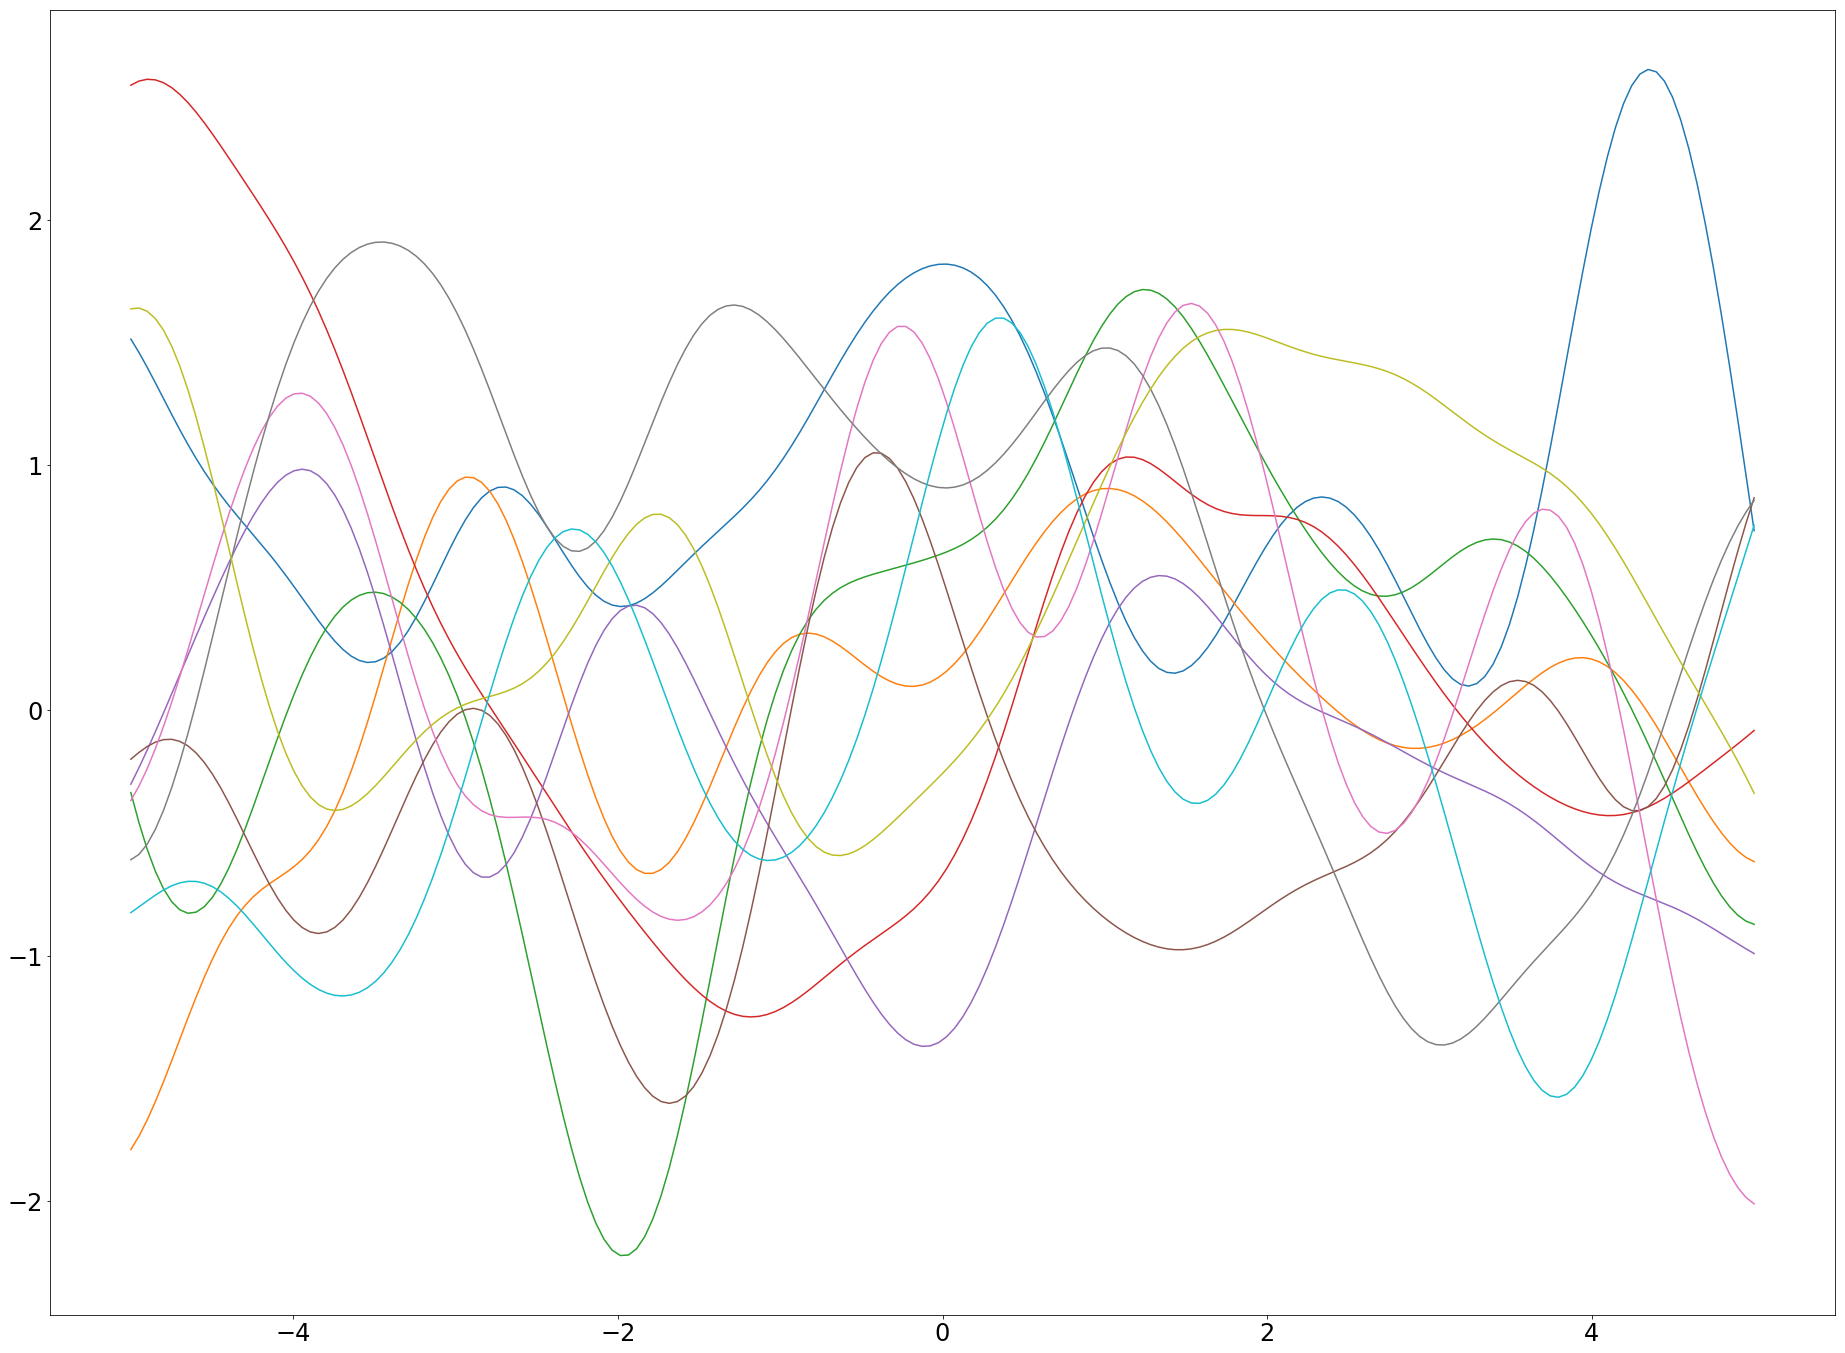
\includegraphics[width=2in,height=1.4in]{lines1}
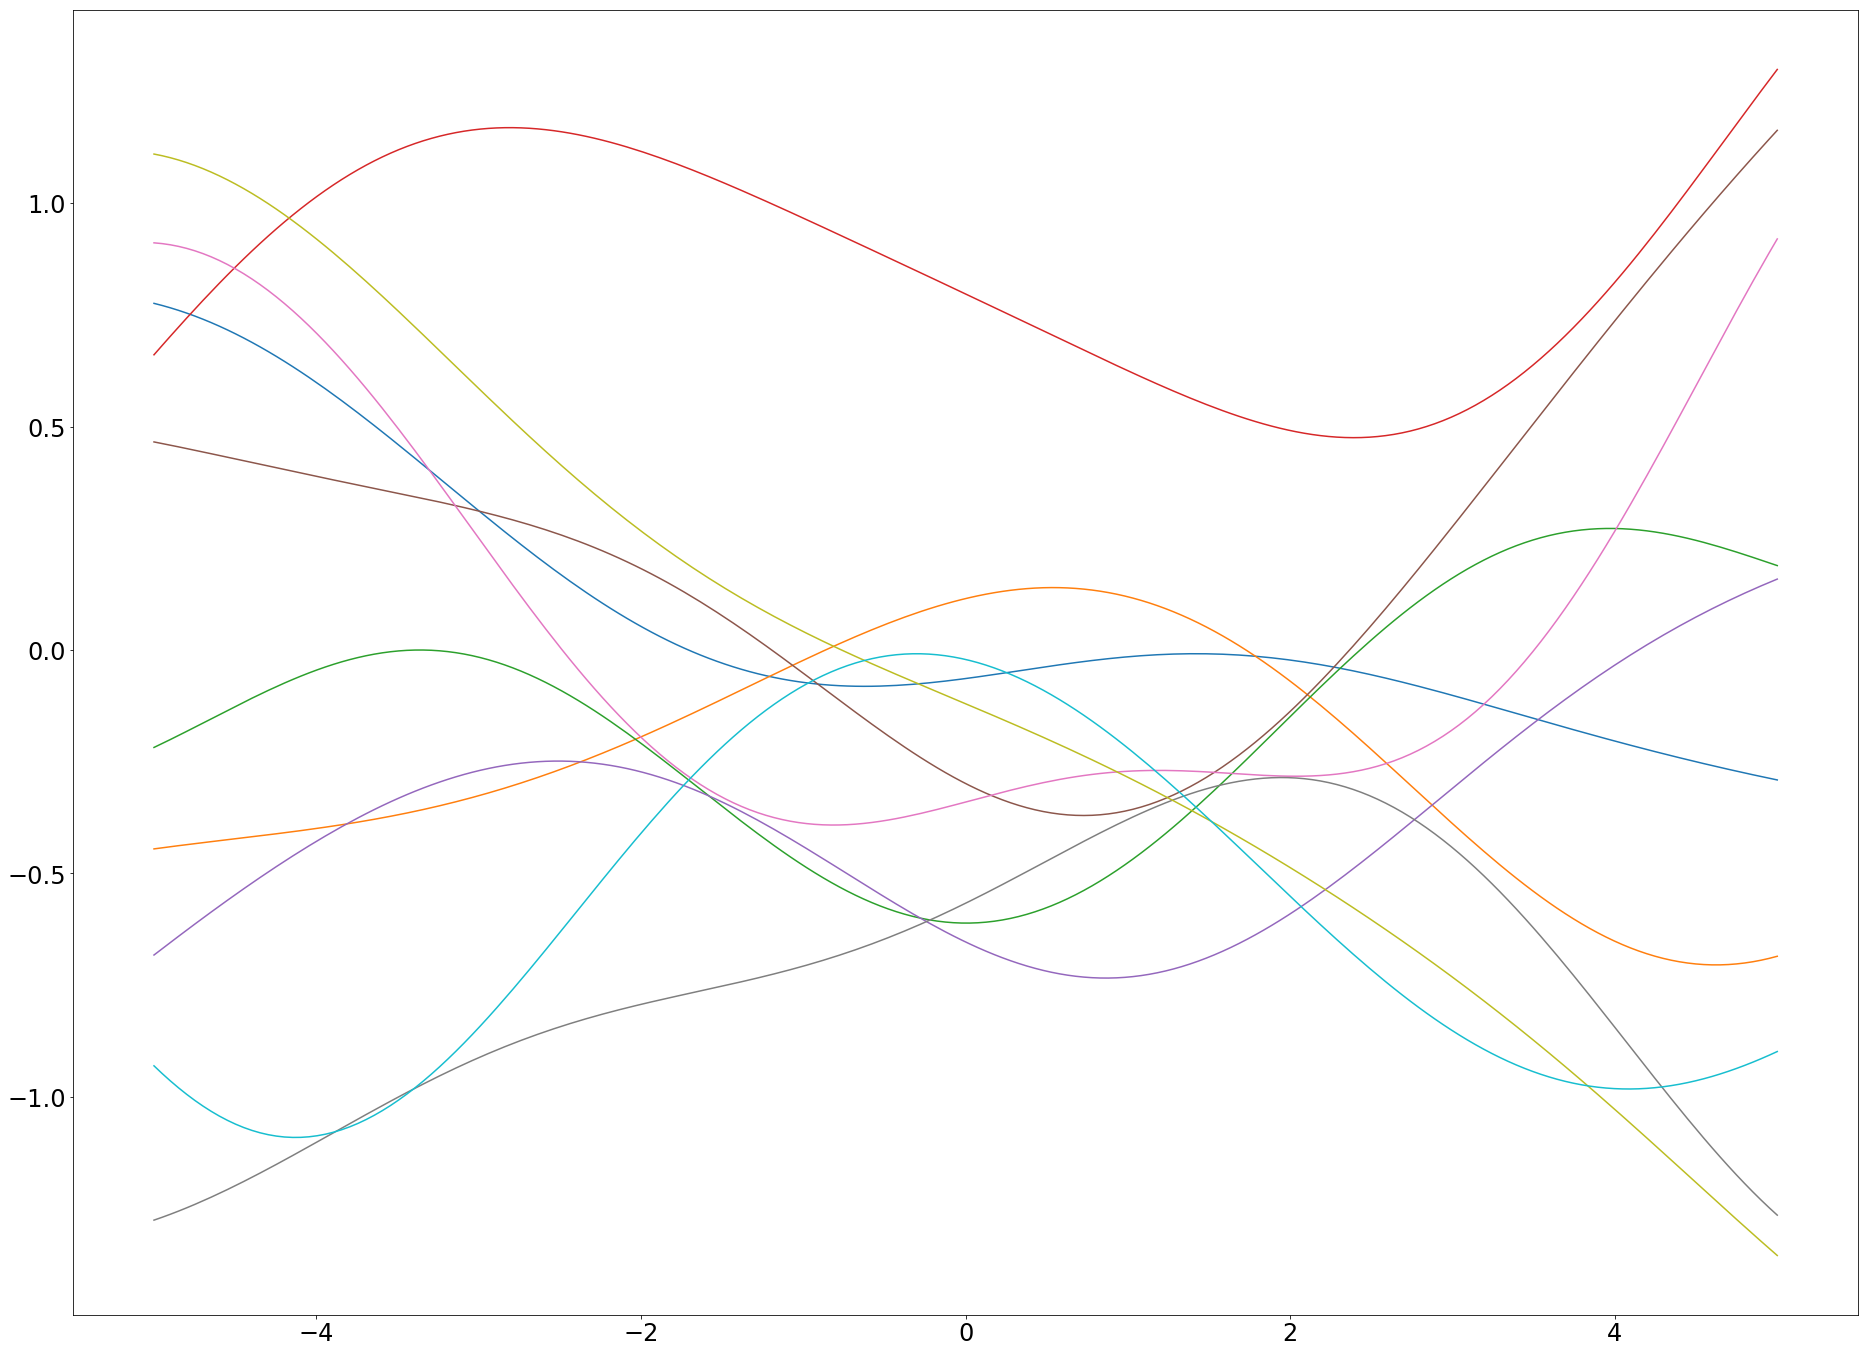
\includegraphics[width=2in,height=1.4in]{lines2}
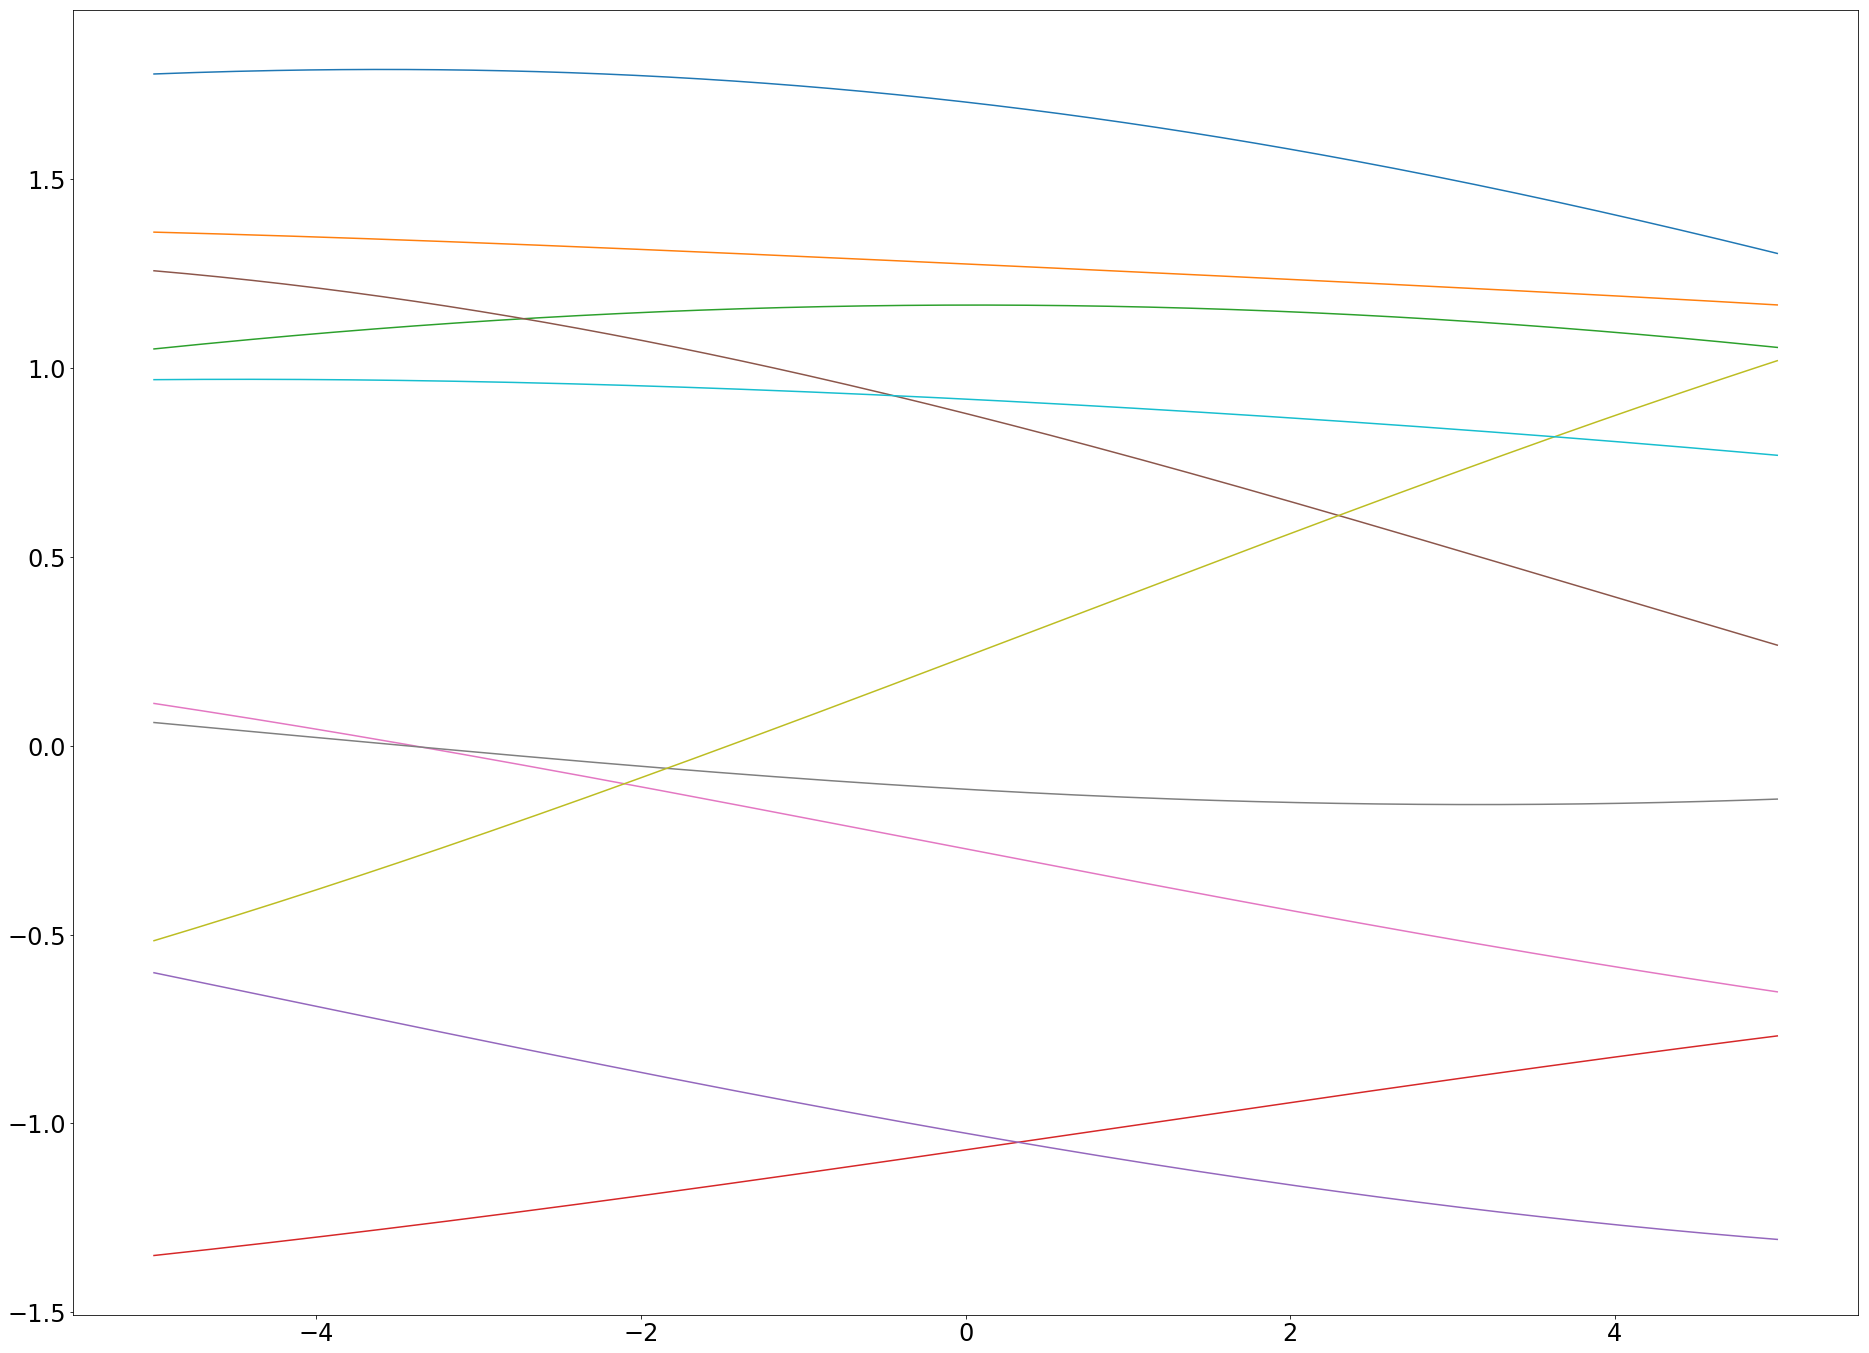
\includegraphics[width=2in,height=1.4in]{lines3} \\

\section*{Question 14}
In question 14 we had to compute the predictive posterior distribution of the model using our aforementioned kernel function.
First we plotted the given 7 points of data against their noisy function evaluation, and plotted behind it a non-noisy sin curve for comparison. Then we sampled from our calculated posterior all along the axis, both near and far from the data, and plotted it over the original data. As you can see the posterior samples stay fairly close to the original data when near it, but grow largely in variance away from it. \\
This is a good behaviour when function complexity is not well known, but noise is fairly inconsequential. Compared to the prior these samples are extremely jagged, however they better represent the data, as the prior samples were completely irrelevant to the data. \\
You can see the plot of the predictive mean and variance below, as you can see variance in the posterior is heavily affected by the presence of real data points, and returns to a uniform gaussian away from them. \\
\newline
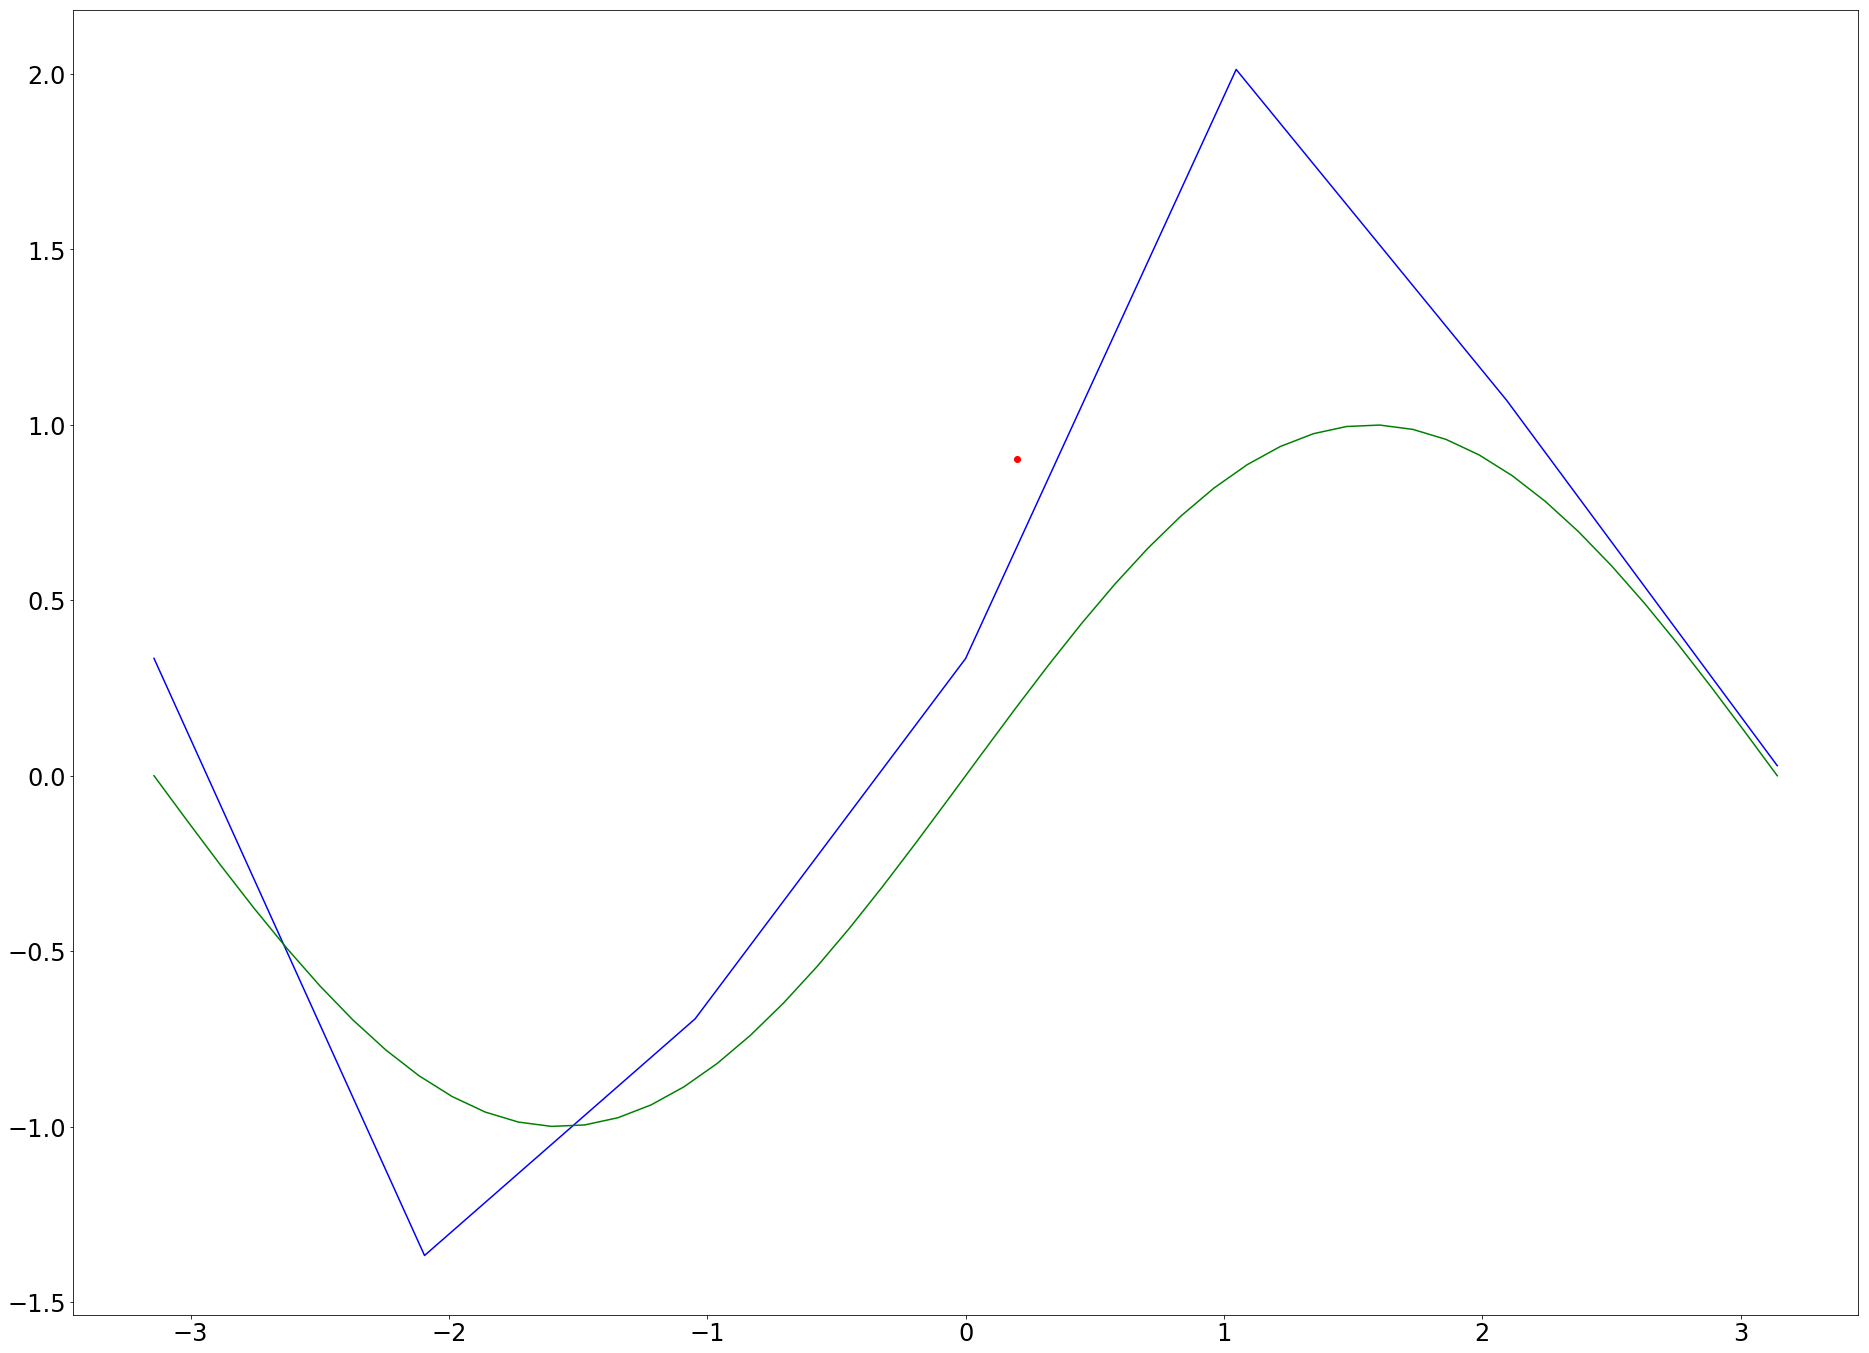
\includegraphics[width=2in,height=1.4in]{curve1}
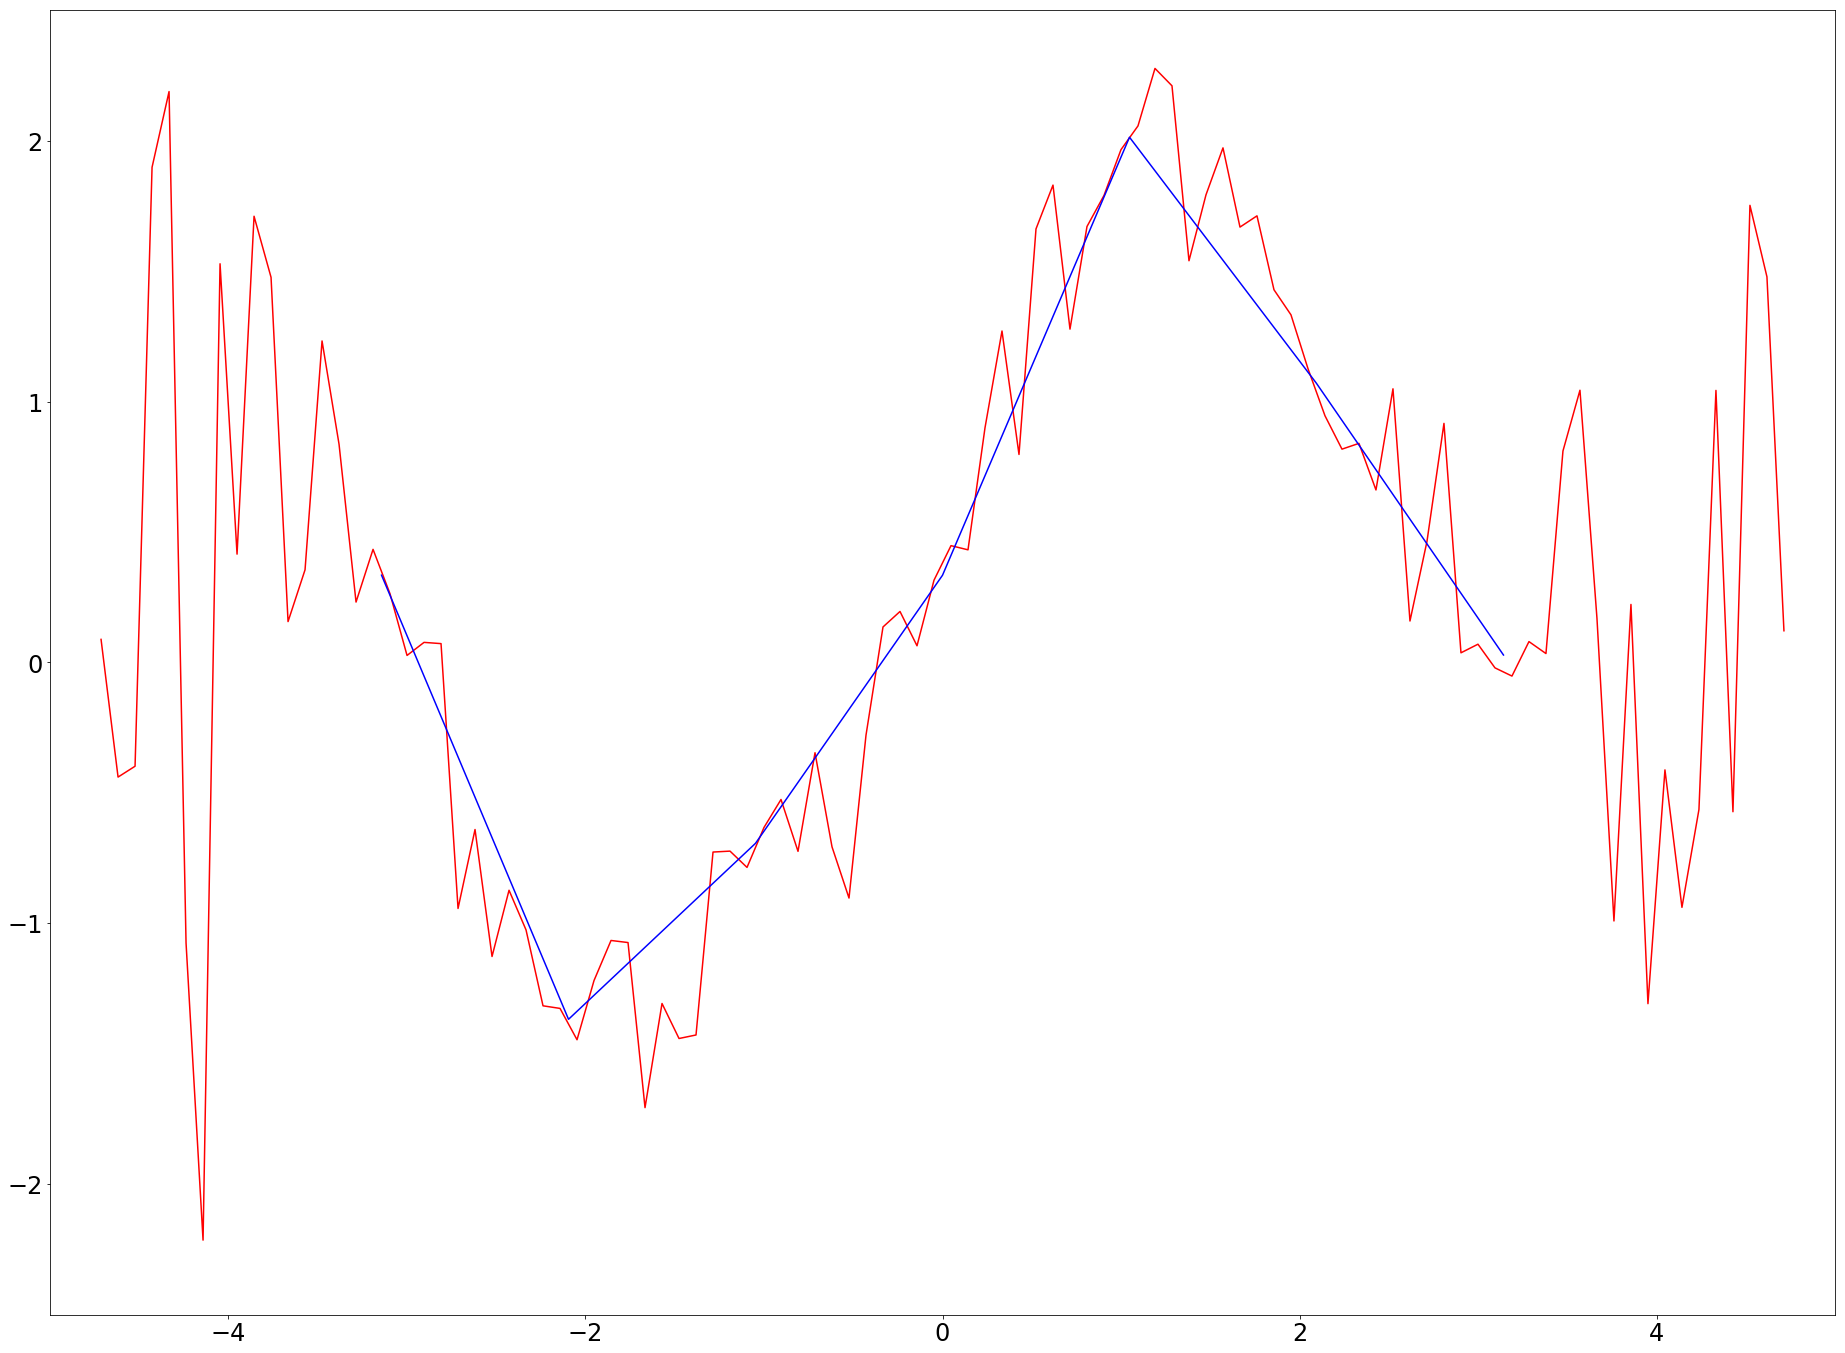
\includegraphics[width=2in,height=1.4in]{curve2}
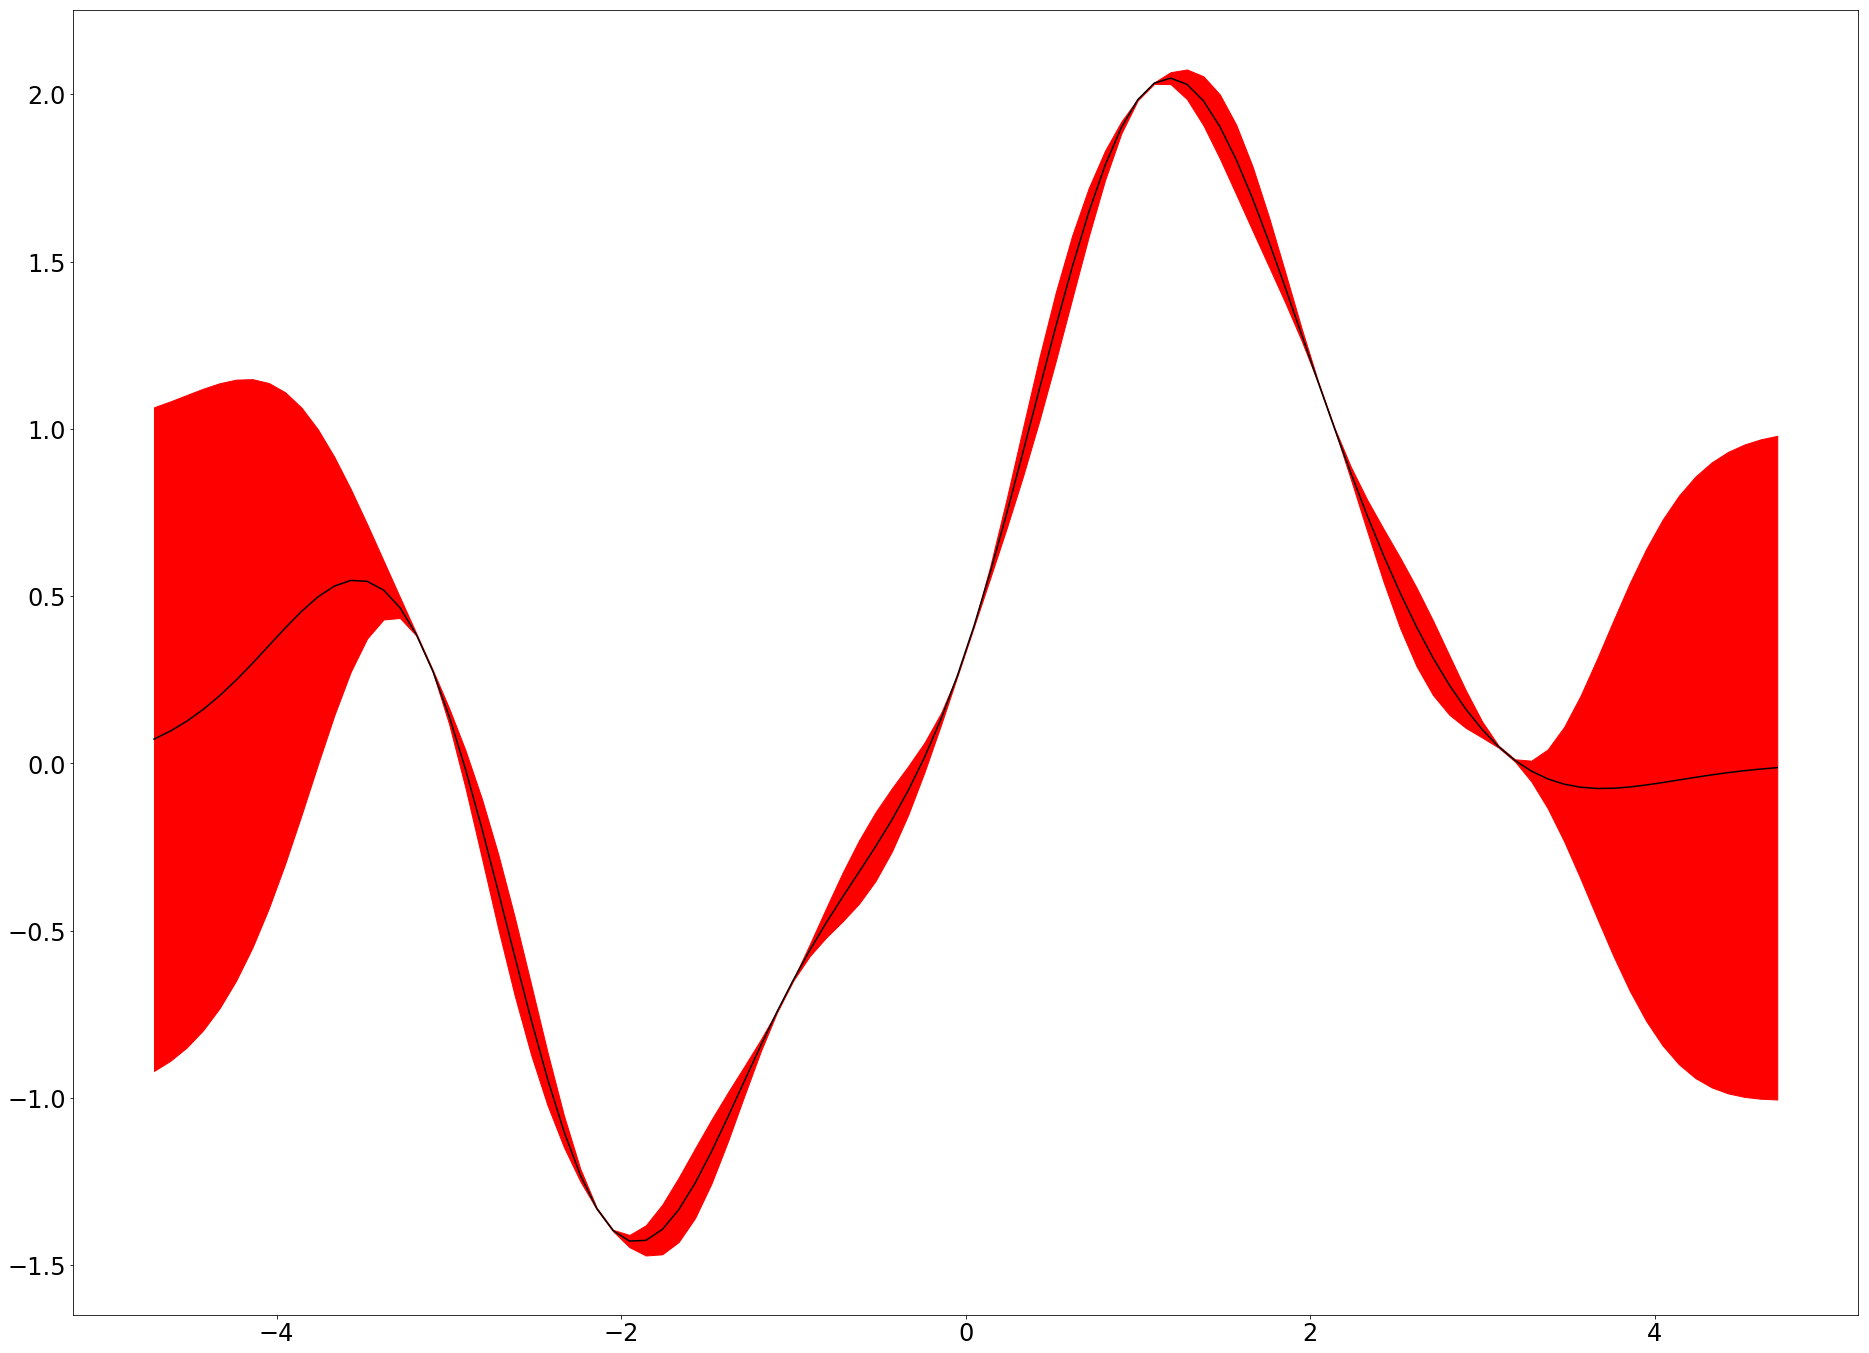
\includegraphics[width=2in,height=1.4in]{curve3} \\

\section*{Question 15}
\subsection*{Elaborate on the relationship between assumptions and preference}
The assumption and preference are subtly different ways of expressing a similar idea; which word we choose to use is contextual. Both assumptions and preferences let you create a prior over some data. However, making an assumption over all the data in a generic way is an assumption, but wanting the model to fit a certain distribution and then encoding the prior in this form is a preference - we are saying what we want to see and not what think we'll see. A preference over a variable we don?t care about can be differentiated and encoded to create a prior that marginalises said variable.

\section*{Question 16}
\subsection*{What is the assumption/preference encoded with the prior?}
The latent variables are only implied and not actually encoded in the data explicitly, instead they are used to reduce the dimensionality of the data. It is in our best interests to keep this as simple as possible, thus we choose to assume that there that our latent variables are independent (have no covariance), vary equally, and have a mean of 0.

\section*{Question 17}
\subsection*{Perform the marginalisation.}
Our prior is \( p(x) = N (0, I) \). We know that our y is some distribution over x plus some error so \\

 \( y = f(x) + \epsilon \) \\

 If we assume our distribution is linear, we can say that \( f(x) = wx \), so \( y = wx + \epsilon \). \\
As the only term in y that varies is \( \epsilon \) we know that our mean is wx, thus we can derive a Gaussian as follows : \\

\( N (wx, \epsilon) \) \\

As we have already assumed that out error is a spherical matrix we know that it is something proportional to the identity matrix, so we can say it is \( \sigma^2 I \). \\
Now we can formulate this with some Gaussian identities to form the prior with x being marginalised: \\

\( P(Y \mid W) = \int N(wx, \sigma^2) N(0, I) = N(0, \sigma^2 I + WW^T) \)

\section*{Question 18}
\subsection*{How do the ML, ML-type II and MAP differ}
The maximum likelihood allows us to formulate and maximise the likelihood of the data by finding parameters. \\
Type II maximum likelihood is an expansion on ML which requires us to first integrate out either the weights of the mapping or the latent representation; then maximise the remaining variables; essentially applying Bayes on half of the probability to allow us to optimise that half while ignoring the other. Type II maximum likelihood is used for unsupervised learning problems, as they?re just too complex to use MAP on. \\
Maximum-a-posteriori estimations require us to maximise the posterior rather than the likelihood, which requires the addition of a prior distribution; thus MAP estimation can be viewed as a regularisation of ML estimation. \\
The difference between the three is the expression they maximise; the ML maximises the likelihood, type-II ML maximises a marginal, and MAP maximises the posterior.
\subsection*{How do MAP and ML differ when we observe more data?}
The main difference for large datasets is that the MAP result will be influenced by a prior while the ML estimation will only be based on the data - provided our prior is good, MAP will generally give us a slightly better result.
\subsection*{Why are the two expressions in Eq. 8 equal?}
he expressions are equal as the integration in the denominator integrates to 1; this is because marginalising out W gives us the probability of every possible occurrence, which is obviously 1.

\section*{Question 19}
The objective function is: \\
\( \mathcal{L} (\mathbf{W}) = constant + log\mid \mathbf{C}(\mathbf{W})\mid + \sum\limits_{i}^N y_{i}^{T}(\mathbf{C}(\mathbf{W}))^{-1} y_{i} \) \\
\newline
To simplify the derivation, we need to remove the sum, we can do this by changing L(W) to matrix form. \\

\( \sum\limits_i x_{i}x_{i} = tr([\leftarrow x_{1} \rightarrow.........\leftarrow x_{N} \rightarrow][\leftarrow x_{1} \rightarrow.........\leftarrow x_{N} \rightarrow]^{T}) \) \\
\newline
As such the equation can be rewritten: \\

\( \mathcal{L}(\mathbf{W}) = constant + log\mid \mathbf{C}(\mathbf{W})\mid + tr(Y(\mathbf{C}(\mathbf{W}))^{-1}Y^T) \) \\
\newline
C is a principle component of the equation, so we need to know how to derive it.\\

\( \frac{\delta C}{\delta W_{ij}} = \frac{\delta WW^T}{\delta W_{ij}} \) \\
\newline
Using Matrix Cookbook, which are just matrix rules, we can get the following derivative: \\

\( \frac{\delta WW^T}{\delta W_{ij}} = W\frac{\delta W^T}{\delta W_{ij}} + \frac{\delta W}{\delta W_{ij}} W^T = WJ_{ij}W^T \) \\

Where \( J_{ij} \) is a matrix where all entries are zero apart from at ij \\
\newline
Now we just need to derive the remaining terms: \\

\( \frac{\delta}{\delta W_{ij}} Log \mid C \mid \) \\
\newline
Using more rules \\

\( \frac{\delta}{\delta W_{ij}} Log \mid C \mid = tr(C^{-1} \frac{\delta C}{\delta W_{ij}} \) \\
\newline
Now for the second term: \\

\( tr(Y (\mathbf{C}(\mathbf{W})^{-1}Y^T) \) \\
\newline
This becomes: \\

\( tr(\frac{\delta}{\delta W_{ij}} Y(C)^{-1}Y^T) \) \\
\newline
Now we can use the chain rule to break the quadratic form: \\

\( tr(\frac{\delta}{\delta W_{ij}} Y(C)^{-1}Y^T) = tr(\frac{\delta}{\delta C} (Y(C)^{-1}Y^T) \frac{\delta C^{-1}}{\delta W_{ij}} ) \) \\
\newline
Now we have the derivative all alone, so: \\

\( tr(Y Y^T \frac{\delta C^{-1}}{\delta W_{ij}}) = tr(Y Y^T ( -C^{-1} \frac{\delta C}{\delta W_{ij}} C^{-1})) \)

\section*{Question 20}
\subsection*{Why is the marginalisation of f simpler to do than marginalise out X}
It's easier to marginalise f because f is only depended on by y, while x is depended on by f and y which makes the calculation much messier. F just contains the uncertainty, which when we marginalise it filters through the rest of the equation. (Refer to Fig .1 in Question 10)

\section*{Question 21}
When trying to recover our input from an output that has had a non-linear, then a linear function applied to it, we can easily recover the inputs to the linear function, not so much for the non-linear one; So the best we can do is recover the output of the non-linear function. What has been plotted is the dot product between our starting data and our recovered data; the x data in 2 dimensions.\\
The output is of a spiral form as we are plotting \(sin\) against \(cos\). The x we have recovered was generated by a non-linear function; each point on the x axis corresponds to multiple y values.
\begin{figure}[H]
\begin{center}
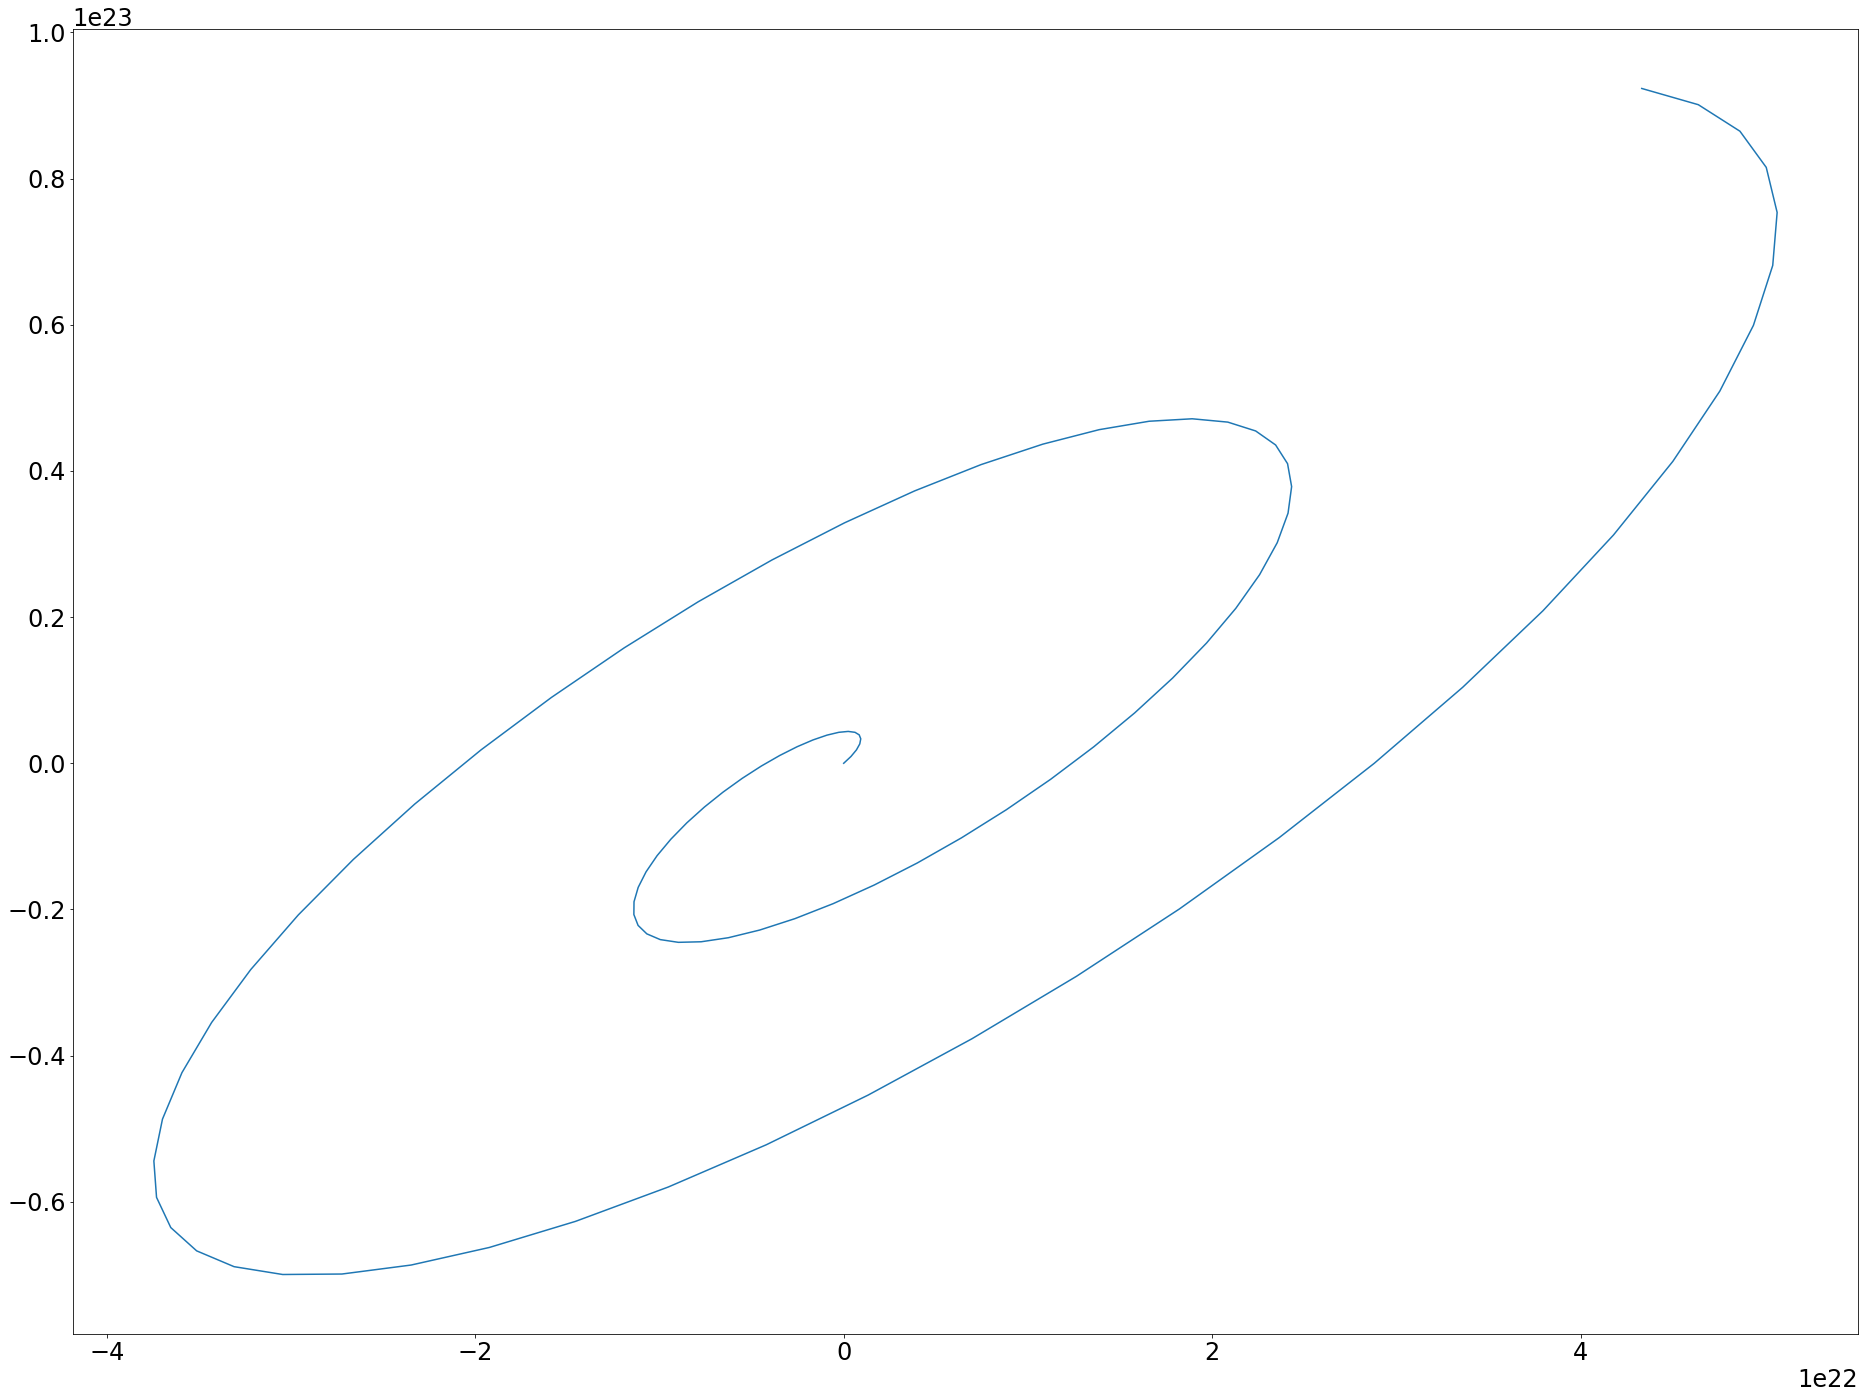
\includegraphics[width=2.2in,height=1.5in]{spiral}
\end{center}
\caption{PCA 10 Dimensions to 2}
\end{figure}

\section*{Question 22}
\subsection*{Why is it the simplest model and what does it imply?}
This assumption implies that each of the 512 elements have an equal probability of occurring.
This is the simplest possible model because we're just assuming that none of the elements are unique, all of them have the exact same probability of occurring and thus our calculation ought to be simple.
\subsection*{Why is it the most complex model?}
It is the most complex model as it attempts to spread the probability mass over the entire dataset space because it places a uniform probability mass over the entire space. This could be an issue as it can penalised by Bayes Rule.

\section*{Question 30}
\subsection*{What have we learnt?}
We have learnt about both parametric and non-parametric models, and in what scenarios to apply them. We have also learnt the importance of uncertainty and assumptions when deriving priors and posteriors; a bad assumption, is very quickly proven to be bad when observing the posterior! We feel that the purpose of this assignment was to give us a hands on approach to machine learning where we can understand some of the core concepts at more than a purely abstract and theoretical level but still using simple and ideal scenarios so we can easily see the outcomes and importance of different concepts. However we must keep in mind that real world scenarios are unlikely to be presented so nicely, and that data will often be presented in a muddled or obscured state.

\end{document}
